\documentclass{article}
\input{article_preamble.tex}

\usepackage{color, soul}
\newcommand{\FC}[1]{{\color{blue} [FC: #1] }}
\newcommand{\KR}[1]{{\color{purple} [KR: #1] }}
\newcommand{\UK}[1]{{\color{orange} [UK: #1] }}
\newcommand{\ZS}[1]{{\color{red} [Zach: #1] }}
\newcommand{\itemdone}{\item[\checkmark]}
\newcommand{\I}{\mathcal{I}}
\newcommand{\J}{\mathcal{J}}

\newcommand{\policies}{{\text{POLICIES}}}
\newcommand{\model}{{\bf (DMO) }}
\newcommand{\modelvax}{{\bf (DMOV) }}


\title{
    Pandemic Mitigation Optimization
}
% \author{\textsc{
%     Uday Karmarkar, Kumar Rajaram, Francisco Castro}\\
%     \normalsize  UCLA Anderson School of Management
% }
% \date{}

\begin{document}
% \maketitle
\maketitleunfinished



% \begin{abstract}
%     \noindent
%     \ZS{Please feel free to add comments inline!}\\
%     \UK{Using the \console{\UK{}} command!}\\
%     \KR{Using the \console{\KR{}} command!}\\
%     \FC{Using the \console{\FC{}} command!}\\
% \end{abstract}

\tableofcontents
% % \newpage


\section{Model}




\subsection{SIRD Model with Variable-Cost Interventions}\label{subsec:SIRD_model}
\subsubsection*{Parameters}

\begin{itemize}
    \item Suppose there are $N$ total individuals, of whom $I_0$ are initially infected. There are $m$ interventions to consider, each of which has (up to) $n$ levels of intensity.
    \item Let $A_{ijt}$ denote the fixed cost of implementing policy $i$ at level $j$ at time $t$.
    \item Let $B_{ijt}$ denote the \emph{switching} cost of implementing policy $i$ at level $j$ at time $t$ (only incurred if policy not implemented in previous period).
    \item Let $C_{ijt}$ denote the per-susceptible-individual cost of implementing poilcy $i$ at level $j$ at time $t$.
    \item Let $C_{infection}$ and $C_{death}$ denote the costs associated with a single individual being infected in a given period, and a single individual losing their life due to disease, respectively.
    \item Let $K_I$ correspond to the infection rate such that the number of new infections is proportional to $K_I$ multiplied by the number of interactions between susceptible and infected individuals, modeled as the product of the sizes of those populations.
    \item  Let $K_R$ and $K_D$ denote the proportion of infected individuals in each period who recover and die, respectively.
    \item Let $P_{ijt}$ denote the factor by which new infections are decreased in period $t$ as a result of implementing policy $i$ at level $j$. In this model, these factors are independent of one another should multiple policies be implemented simultaneously.
\end{itemize}

\subsubsection*{Decision Variables}
\begin{itemize}
    \item Let
          \begin{equation}\label{eq:y_definition}\tag{8a}
              y_{ijt} = \begin{cases}1 &: \parbox[c]{8cm}{policy $i$ is implemented at level $j$ in time period $t$}\\ 0 &: \text{otherwise}\end{cases}
          \end{equation}
    \item Let
            \begin{equation}\label{eq:z_definition}\tag{9a}
                z_{ijt} = \begin{cases}1 &: \parbox[c]{8cm}{policy $i$ is implemented at level $j$ in time period $t$, but not $t-1$}\\ 0 &: \text{otherwise}\end{cases}
            \end{equation}
\end{itemize}

\subsubsection*{State Variables}
\begin{itemize}
    \item Let $S_t, I_t, R_t, d_t$, and $D_t$ denote the population of individuals at time $t$ who are \underline{S}usceptible, \underline{I}nfected, \underline{R}ecovered, \underline{d}ying (in the current period), and \underline{D}ead (cumulatively), respectively. These values depend on the interventions applied.
    \item Let $P_t$ denote the cumulative factor by which new infections are decreased between periods $t-1$ and $t$. That is,
          \begin{equation}\label{eq:Pt_definition}\tag{6a}
              P_t = \prod_{\substack{i,j \text{ s.t.}\\\text{policy $i$ used}\\\text{at level $j$}\\\text{in period $t$}}}P_{ijt}
          \end{equation}

\end{itemize}

\subsubsection*{Model Formulation: Disease Mitigation Optimization \model}\label{subsec:mathprogram}
{\small
    \begin{alignat}{4}
        &\Minimize_{y,P,S,I,R,D,d}\qquad \span\span\span\span \sum_{i=1}^{m}\sum_{j=1}^{n}\sum_{t=1}^{T}A_{ijt} y_{ijt} + B_{ijt}z_{ijt} + C_{ijt} S_{t}  y_{ijt}  + \sum_{t=1}^{T}C_{infection} I_t &&+ C_{death}  d_t \tag{0}\label{eq:objective0}\\
        & \text{s.t.}\qquad  && S_t &&= S_{t-1} - K_I \cdot P_t \cdot S_{t-1} \cdot I_{t-1} && \fa t \in \{2,\ldots,T\} \label{eq:1}\\
        & {} && I_t &&= I_{t-1} + K_I \cdot P_t \cdot S_{t-1} \cdot I_{t-1} - K_R\cdot I_{t-1} - K_D \cdot I_{t-1} && \fa t \in \{2,\ldots,T\} \label{eq:2}\\
        & {} && R_t &&= R_{t-1} + K_R \cdot I_{t-1} && \fa t \in \{2,\ldots,T\} \label{eq:3}\\
        & {} && d_t &&= K_D \cdot I_{t-1} && \fa t \in \{2,\ldots,T\} \label{eq:4}\\
        & {} && D_t &&= D_{t-1} + d_t && \fa t \in \{2,\ldots,T\} \label{eq:5}\\
        & {} && P_t &&= \prod_{i=1}^{m}\prod_{j=1}^{n}\left(1-y_{ijt} + P_{ijt}\cdot y_{ijt}\right)&& \fa t \in \{1,\ldots,T\} \label{eq:6}\\
        & {} && \sum_{j=1}^{n}y_{ijt}  &&\le 1 && \fa i,t \label{eq:7}\\
        & {} && y_{ijt} &&\in \{0,1\} && \fa i,j,t \label{eq:8}\\
        & {} && z_{ijt} &&\ge y_{ij(t)}-y_{ij(t-1)} \text{\qquad(let $y_{ij0}=0 \fa i,j$)} && \fa i,j, t \label{eq:9}\\
        & {} && 0 \le z_{ijt} &&\le 1 && \fa i,j, \fa t\ge 1 \label{eq:10}\\
        & {} && I_1 &&= I_0 && \nonumber\\
        & {} && S_1 &&= N - I_0 && \nonumber\\
        & {} && D_1 &&= 0 && \nonumber\\
        & {} && R_1 &&= 0 && \nonumber\\
        & {} && d_1 &&= 0 && \nonumber
    \end{alignat}
}


The objective function \eqref{eq:objective0} is the sum of the costs of implementing the policy interventions in all periods and the costs associated with the resulting disease and death in all periods (due to lost productivity and resources).

The constraints \eqref{eq:1},\eqref{eq:2},\eqref{eq:3},\eqref{eq:4}, and \eqref{eq:5} model the SIRD compartment subpopulations as the disease progresses alongside the infection-reduction factors $P_t$ at each period $t=1,\ldots,T$. The constraint \eqref{eq:6} models the multiplicative effect of multiple interventions being applied in the same period, as described by \eqref{eq:Pt_definition}. Equation \eqref{eq:7} enforces the logical constraint that at most one level from each policy be used in each period, and \eqref{eq:8} ensures that the $y_{ijt}$ variables correspond to the binary definition in \eqref{eq:y_definition}.




\subsection{SIRD Model with Non-Variable-Cost Interventions}

Replace the objective \eqref{eq:objective0} in the mathematical program formulation of the \model model with
\begin{alignat}{3}
   & \Minimize_{y,P,S,I,R,D,d}\qquad \sum_{i=1}^{m}\sum_{j=1}^{n}\sum_{t=1}^{T}A_{ijt}y_{ijt} + B_{ijt}z_{ijt}+ C_{ijt}\cdot &&{\color{red}S_{t}} \cdot y_{ijt}+ \sum_{t=1}^{T}C_{infection}\cdot I_t &&+ C_{death} \cdot d_t \tag{\ref{eq:objective0}}\\
   & &&\mathbf{\Downarrow}\nonumber\\
   & \Minimize_{y,P,S,I,R,D,d}\qquad \sum_{i=1}^{m}\sum_{j=1}^{n}\sum_{t=1}^{T}A_{ijt}y_{ijt} + B_{ijt}z_{ijt}+ C_{ijt}\cdot &&{\color{red}N} \cdot y_{ijt}+ \sum_{t=1}^{T}C_{infection}\cdot I_t &&+ C_{death} \cdot d_t  \label{eq:obj_nonvariable}
\end{alignat}



\subsection{Parameters in Trials}\label{sec:params_table}

All the numerical experiments performed utilized the following parameters:

\begin{figure}[H]
        \begin{center}
        \input{parameters_table.tex}
        \end{center}
        \caption{Policy parameters $P_{ijt}$, $A_{ijt}$, $B_{ijt}$, and $C_{ijt}$ are in general dynamic (time-varying) in the full \model model. In our numerical experiments, we use non-dynamic policies, and in each row of this table corresponding to policy $i$, parameters are listed for each level $j$.}
        \label{table:params}
\end{figure}


\subsection{SIRD Model with Vaccination}

The COVID-19 pandemic demonstrates that a vaccine, which alters disease progression, may become suddenly available within the horizon of intervention decision-making and disease progression. We model vaccination as a change in disease progression when a vaccine becomes available, beginning at time period $T_{vax}$. The value of $T_{vax}$ is exogenous to the model, but can be treated via sensitivity analysis or optimization under uncertain parameters regarding the likelihood of possible vaccine development timelines. We do not treat the ``waning'' of immunity provided by vaccination and assume that vaccination provides a lasting but imperfect reduction in infection and death rates.

The model is modified via the following parameters:
\begin{itemize}
    \item The period $T_{vax}$ is when vaccination becomes available.
    \item The parameters $S_t$ and $I_t$, which represent the number of susceptible and infected individuals in each period, are divided into the following compartments:
    \begin{itemize}
        \item $S_t^{vax}, S_t^{unvax}$, and $S_t^{antivax}$ represent the populations of \emph{vaccinated}, \emph{unvaccinated but willing to be vaccinated}, and \emph{vaccinated and unwilling to be vaccinated} susceptible individuals at time $t$.

        \item Similarly, $I_t^{vax}$ and $I_t^{novax}$ represent the populations of \emph{vaccinated} and \emph{unvaccinated} infected individuals at time $t$. Here, the notation ``novax'' (rather than ``unvax'') reflects that this includes unvaccinated individuals who were previously either willing or unwilling to become vaccinated. Since this model assumes that infection and recovery lead to full immunity, there is no need to distinguish between willingness to become vaccinated among the infected.

        \item The number of newly-vaccinated individuals in period $t$ is $v_t$. \redtext{Lowercase variable to denote ``single-period'' populations not constituting compartments, like $d_t$ (contrasted with $D_t$).}

        \item The proportion of unvaccinated susceptible individuals willing to be vaccinated who become vaccinated in period $t$ is $K_v(t)$. We exclusively model the case in which
        \begin{equation}\label{eq:kvt}
            K_v(t) = \begin{cases}K_v &: \text{$t\ge T_v$}\\ 0 &: \text{otherwise.}\end{cases}
        \end{equation}
        That is, fraction $K_v$ of susceptible unvaccinated individuals ($K_v$ of $S_t^{unvax}$) become vaccinated in each period after $T_v$, and none become vaccinated before that.

    \end{itemize}

    % \item The parameters $P_{ijt}$ and $P_t$, denoting the effect of policy $i$ at level $j$ on infection rate in time period $t$, and the cumulative effect of selected policies, are replaced by parameters $P_{ijt}^{vax}$ and $P_{ijt}^{unvax}$, reflecting the effect of the policy on the two groups.
    \item The infection rate parameter $K_I$ is represented by $K_I^{vax}$ and $K_I^{novax}$, which represents the proportional infection rates of both vaccinated and unvaccinated individuals via the same mixing model.

    \item The recovery and death rate parameters $K_R$ and $K_D$ have vaccinated and unvaccinated variants $K_R^{vax}$, $K_R^{novax}$, $K_D^{vax}$, and $K_D^{novax}$.
\end{itemize}


\subsubsection*{Model Formulation: Disease Mitigation Optimization with Vaccination \modelvax}\label{subsec:mathprogram_vax}

The resulting model can be expressed as follows:


{\small
    \begin{alignat*}{4}
        &\Minimize_{y,P,S^*,I^*,R,D,d,V}\qquad \span\span\span\span \sum_{i=1}^{m}\sum_{j=1}^{n}\sum_{t=1}^{T}A_{ijt} y_{ijt} + B_{ijt}z_{ijt} + C_{ijt} S_{t}  y_{ijt}  + \sum_{t=1}^{T}C_{infection} I_t &&+ C_{death}  d_t \\
        & \text{s.t.}\qquad  && S_t &&= S_t^{vax} + S_{t}^{unvax} + S_t^{antivax}&& \fa t \in \{2,\ldots,T\} \\
        & {} && I_t &&= I_t^{vax} + I_{t}^{novax} && \fa t \in \{2,\ldots,T\} \\
        & {} && S_t^{vax} &&= S_{t-1}^{vax} - K_I^{vax} \cdot P_t \cdot S_{t-1}^{vax} \cdot I_{t-1} + v_t && \fa t \in \{2,\ldots,T\} \\
        & {} && S_t^{unvax} &&= S_{t-1}^{unvax} - K_I^{novax} \cdot P_t \cdot S_{t-1}^{unvax} \cdot I_{t-1} - v_t && \fa t \in \{2,\ldots,T\} \\
        & {} && S_t^{antivax} &&= S_{t-1}^{antivax} - K_I^{novax} \cdot P_t \cdot S_{t-1}^{antivax} \cdot I_{t-1} && \fa t \in \{2,\ldots,T\} \\
        & {} && I_t^{vax} &&= I_{t-1}^{vax} + K_I^{vax} \cdot P_t \cdot S_{t-1}^{vax} \cdot I_{t-1} - K_R^{vax}\cdot I_{t-1}^{vax} - K_D^{vax} \cdot I_{t-1}^{vax} && \fa t \in \{2,\ldots,T\} \\
        & {} && I_t^{novax} &&= I_{t-1}^{novax} + K_I^{novax} \cdot P_t \cdot (S_{t-1}^{unvax} +S_{t-1}^{antivax}) \cdot I_{t-1} - K_R^{novax}\cdot I_{t-1}^{novax} - K_D^{novax} \cdot I_{t-1}^{novax} && \fa t \in \{2,\ldots,T\} \\
        & {} && R_t &&= R_{t-1} + K_R^{vax} \cdot I_{t-1}^{vax} + K_R^{novax} \cdot I_{t-1}^{novax} && \fa t \in \{2,\ldots,T\} \\
        & {} && v_t &&= K_v(t) \cdot S_{t-1}^{unvax} && \fa t \in \{2,\ldots,T\} \\
        & {} && d_t &&= K_D^{vax}\cdot I_{t-1}^{vax} + K_D^{unvax} \cdot I_{t-1}^{unvax} && \fa t \in \{2,\ldots,T\} \\
        & {} && D_t &&= D_{t-1} + d_t && \fa t \in \{2,\ldots,T\} \\
        & {} && P_t &&= \prod_{i=1}^{m}\prod_{j=1}^{n}\left(1-y_{ijt} + P_{ijt}\cdot y_{ijt}\right)&& \fa t \in \{1,\ldots,T\} \\
        & {} && \sum_{j=1}^{n}y_{ijt}  &&\le 1 && \fa i,t \\
        & {} && y_{ijt} &&\in \{0,1\} && \fa i,j,t \\
        & {} && z_{ijt} &&\ge y_{ij(t)}-y_{ij(t-1)} \text{\qquad(let $y_{ij0}=0 \fa i,j$)} && \fa i,j, t \\
        & {} && 0 \le z_{ijt} &&\le 1 && \fa i,j, \fa t\ge 1 \\
        & {} && I_1 = I_1^{novax}  &&= I_0 && \\
        & {} && S_1 &&= N - I_0 && \\
        & {} && S_1^{vax}, S_1^{antivax} &&= 0, S_0^{antivax} && \\
        & {} && D_1 &&= 0 && \\
        & {} && R_1 &&= 0 && \\
        & {} && d_1 &&= 0 &&
    \end{alignat*}
}



\section{Heuristics}

\subsection{Lagrangian Heuristic and Lower Bound}\label{sec:lagrangian}

We can utilize a Lagrangian relaxation to the full problem \model by relaxing constraints \eqref{eq:6} and instead penalizing the objective function using dual multipliers. The relaxed problem decomposes into two computationally less expensive subproblems; by iteratively updating the multipliers using gradient ascent, the lower bound tightens. Furthermore, we can transform a solution to the relaxed problem into a feasible solution for the full problem, yielding a heuristic solution in its own right.

First, we focus on the variant of the model in which interventions do not have a variable cost depending on the size of the susceptible population ($S_t$), and instead have a ``variable'' cost proportional to the size of the entire population ($N$), as in \eqref{eq:obj_nonvariable} (i.e., the costs do not ``vary'' between time periods). This allows the Lagrangian minimization problem to be split into two subproblems.

Then, we transform constraint \eqref{eq:6} using a logarithm:
\begin{equation}\label{eq:6log}\tag{\ref{eq:6}-$\log$}
    \ln P_t = \sum_{i=1}^{m}\sum_{j=1}^{n} \ln (1-y_{ijt} + P_{ijt} y_{ijt}), \fa t=1,\ldots,T.
\end{equation}
Next, we remove this constraint from \model and augment the objective \eqref{eq:obj_nonvariable} via multipliers $\lambda_t,t=1,\ldots,T$ to obtain a relaxed minimization problem:
{\small
    \begin{alignat}{4}
        &\Minimize_{y,P,S,I,R,D,d}\qquad &&&& \left[\text{Objective \eqref{eq:obj_nonvariable}}\right] + \sum_{t=1}^{T}\lambda_t \left(\sum_{i=1}^{m}\sum_{j=1}^{n} \ln (1-y_{ijt} + P_{ijt} y_{ijt})- \ln P_t\right)\label{eq:lagrangian_obj}\\
        &  \text{s.t.} && 0 \le P_t &&\le 1 \label{eq:extra_constraint}\\
        &   &&  &&\text{Constraints from \model except for \eqref{eq:6}.}\nonumber
    \end{alignat}
}
An optimal value to the augmented problem \eqref{eq:lagrangian_obj} is a lower bound to the optimal value of the full problem \model. We add an extra constraint \eqref{eq:extra_constraint} to enforce the logical constraints that the policy effectiveness factors are between $0$ and $1$; note that in a numerical implementation, it may actually be preferable to precompute a reasonable lower bound on $\underline{P}_t \in (0,1)$ and constrain $\underline{P}_t \le P_t \le 1$ because the logarithm in \eqref{eq:lagrangian_obj} is undefined for $P_t=0$.

By iteratively solving the augmented problem \eqref{eq:lagrangian_obj} and then using subgradient ascent to update $\lambda_t$ for all $t=1,\ldots,T$, we obtain increasingly tighter lower bounds on the optimal value for the full problem \model.


Note that the augmented problem \eqref{eq:lagrangian_obj} can be decomposed into two minimization problems with optimal values $L_1(\bm{\lambda})$ and $L_2(\bm{\lambda})$:\\
\begin{minipage}{\linewidth}
{
    $L_1(\bm{\lambda})$ is the solution to\\
    \small
    \begin{alignat}{4}
        &\Minimize_{y}\qquad \span\span\span\span\span\span \sum_{i=1}^{m}\sum_{j=1}^{n}\sum_{t=1}^{T} \left[A_{ijt}\cdot y_{ijt} + B_{ijt}z_{ijt} + C_{ijt}\cdot N \cdot y_{ijt}  + \lambda_t \ln (1-y_{ijt} + P_{ijt} y_{ijt}) \right]\nonumber\\
        % & \text{s.t.} \qquad&& S_t &&= S_{t-1} - K_I \cdot P_t \cdot S_{t-1} \cdot I_{t-1} && \fa t \in \{2,\ldots,T\} \tag{\ref{eq:1}}\\
        %  & {} && I_t &&= I_{t-1} + K_I \cdot P_t \cdot S_{t-1} \cdot I_{t-1} - K_R\cdot I_{t-1} - K_D \cdot I_{t-1} && \fa t \in \{2,\ldots,T\} \tag{\ref{eq:2}}\\
        %  & {} && R_t &&= R_{t-1} + K_R \cdot I_{t-1} && \fa t \in \{2,\ldots,T\} \tag{\ref{eq:3}}\\
        %  & {} && d_t &&= K_D \cdot I_{t-1} && \fa t \in \{2,\ldots,T\} \tag{\ref{eq:4}}\\
        %  & {} && D_t &&= D_{t-1} + d_t && \fa t \in \{2,\ldots,T\} \tag{\ref{eq:5}}\\
         & {} && \sum_{j=1}^{n}y_{ijt}  &&\le 1 && \fa i,t \tag{\ref{eq:7}}\\
         & {} && y_{ijt} &&\in \{0,1\} && \fa i,j,t \tag{\ref{eq:8}}\\
         & {} && z_{ijt} &&\ge y_{ij(t)}-y_{ij(t-1)}  && \fa i,j, t \tag{\ref{eq:9}}\\
         & {} && 0 \le z_{ijt} &&\le 1 && \fa i,j, \fa t\ge 1 \tag{\ref{eq:10}}
        % & {} && I_1 &&= I_0 && \nonumber\\
        % & {} && S_1 &&= N - I_0 && \nonumber\\
        % & {} && D_1 &&= 0 && \nonumber\\
        % & {} && R_1 &&= 0 && \nonumber\\
        % & {} && d_1 &&= 0 && \nonumber
    \end{alignat}
}

This integer program can be solved by standard off-the-shelf software such as Gurobi.

\redtext{Note: Nonlinear integer programs have only been solvable by Gurobi \href{https://www.gurobi.com/wp-content/uploads/2019/12/Gurobi-9.0-Overview-Webinar-Slides-1.pdf}{since November 2019}. I wonder whether there is a more complete explanation of why this subproblem is in fact ``easier" than the full problem.}
\end{minipage}\\

\begin{minipage}{\linewidth}
{
    $L_2(\bm{\lambda})$ is the solution to\\
    \small
    \begin{alignat}{4}
        &\Minimize_{P,S,I,R,D,d}\qquad \span\span\span\span\span \sum_{t=1}^{T}\left[C_{infection}\cdot I_t + C_{death} \cdot d_t -\lambda_t \ln P_t\right]\nonumber\\
        & \text{s.t.} \qquad&& S_t &&= S_{t-1} - K_I \cdot P_t \cdot S_{t-1} \cdot I_{t-1} && \fa t \in \{2,\ldots,T\} \tag{\ref{eq:1}}\\
        & {} && I_t &&= I_{t-1} + K_I \cdot P_t \cdot S_{t-1} \cdot I_{t-1} - K_R\cdot I_{t-1} - K_D \cdot I_{t-1} && \fa t \in \{2,\ldots,T\} \tag{\ref{eq:2}}\\
        & {} && R_t &&= R_{t-1} + K_R \cdot I_{t-1} && \fa t \in \{2,\ldots,T\} \tag{\ref{eq:3}}\\
        & {} && d_t &&= K_D \cdot I_{t-1} && \fa t \in \{2,\ldots,T\} \tag{\ref{eq:4}}\\
        & {} && D_t &&= D_{t-1} + d_t && \fa t \in \{2,\ldots,T\} \tag{\ref{eq:5}}\\
        % & \text{s.t.} && \sum_{j=1}^{n}y_{ijt}  &&\le 1 && \fa i,t \tag{\ref{eq:7}}\\
        % & {} && y_{ijt} &&\in \{0,1\} && \fa i,j,t \tag{\ref{eq:8}}\\
        & && P_t &&\le 1 \tag{\ref{eq:extra_constraint}}\\
        & {} && I_1 &&= I_0 && \nonumber\\
        & {} && S_1 &&= N - I_0 && \nonumber\\
        & {} && D_1 &&= 0 && \nonumber\\
        & {} && R_1 &&= 0 && \nonumber\\
        & {} && d_1 &&= 0 && \nonumber
    \end{alignat}
}
This problem has no integer constraints and can be solved by any nonlinear programming software.
\end{minipage}

To increase the tightness of the bound in the gradient-ascent step for the multipliers $\bm{\lambda}$, where $\bm{\lambda}^+$ represents the vector of multipliers at a subsequent iteration, we use the updating rule:
\[
    \bm{\lambda}^+ = \bm{\lambda} + \gamma \left(\nabla L_1(\bm{\lambda}) + \nabla L_2(\bm{\lambda})\right),
\]
i.e.
\begin{equation}\label{eq:lambda_update}
    \lambda_t^+ = \lambda_t + \gamma \cdot  \left(\sum_{i=1}^{m}\sum_{j=1}^{n} \ln (1-y_{ijt} + P_{ijt} y_{ijt})- \ln P_t\right).
\end{equation}

To obtain a feasible solution to the full problem \model after any iteration of this procedure, one can fix the values of $y_{ijt}, i=1,\ldots,m,j=1,\ldots,n,t=1,\ldots,T$ in \model to those obtained in the decomposed minimizations, which immediately yields values of $P_t,t=1,\ldots,T$, which in turn gives values of the compartment subpopulations ($S,I,R,d,$ and $D$) following basic bookkeeping.

This procedure can be iteratively performed indefinitely, and will yield a sequence of nondecreasing lower bounds to the full problem \model. As a stopping criterion, one can terminate when the relative improvement between two iterations is less than a threshold (``improvement''), or when the relative optimality gap between the incumbent feasible solution and the greatest lower bound is less than a threshold (``optimality gap''). More formally, the heuristic corresponding to this procedure can be described as follows:
\begin{pseudocode}
    Initialize |$\lambda_t\leftarrow0$| for all t.
    Do
       Minimize to obtain |$L_1(\bm{\lambda})$| and |$L_2(\bm{\lambda})$|
       Update |$\bm{\lambda}$| via gradient ascent as in |\eqref{eq:lambda_update}|
       The value |$L_1(\bm{\lambda}) + L_2(\bm{\lambda})$| gives a lower bound.
       The optimal values of |$y_{ijt}$| from |$L_1(\bm{\lambda})$| substituted in the original problem |\model| yield a feasible solution and thus an upper bound for that problem's optimal solution.
    Repeat while stopping condition (improvement or optimality gap) is not met.
\end{pseudocode}


\subsubsection{Lagrangian Heuristic and Lower Bound for the Vaccination Model}

The Lagrangian of the variation of \model model that includes vaccination, as in \eqref{subsec:mathprogram_vax}, can again be decomposed into two minimization problems with optimal values $L_1^{vax}(\bm{\lambda})$ and $L_2^{vax}(\bm{\lambda})$, where, for any value of $\bm{\lambda}\ge0$, $L_1^{vax}(\bm{\lambda}) + L_2^{vax}(\bm{\lambda})$ yields a lower bound on the problem \eqref{subsec:mathprogram_vax}:

{\small
    \begin{alignat*}{4}
        &\Minimize_{y,P,S^*,I^*,R,D,d,V}\qquad \span\span\span\span \sum_{i=1}^{m}\sum_{j=1}^{n}\sum_{t=1}^{T}A_{ijt} y_{ijt} + B_{ijt}z_{ijt} + C_{ijt} S_{t}  y_{ijt}  + \sum_{t=1}^{T}C_{infection} I_t &&+ C_{death}  d_t \\
        & \text{s.t.}\qquad  && S_t &&= S_t^{vax} + S_{t}^{unvax} + S_t^{antivax}&& \fa t \in \{2,\ldots,T\} \\
        & {} && I_t &&= I_t^{vax} + I_{t}^{novax} && \fa t \in \{2,\ldots,T\} \\
        & {} && S_t^{vax} &&= S_{t-1}^{vax} - K_I^{vax} \cdot P_t \cdot S_{t-1}^{vax} \cdot I_{t-1} + v_t && \fa t \in \{2,\ldots,T\} \\
        & {} && S_t^{unvax} &&= S_{t-1}^{unvax} - K_I^{novax} \cdot P_t \cdot S_{t-1}^{unvax} \cdot I_{t-1} - v_t && \fa t \in \{2,\ldots,T\} \\
        & {} && S_t^{antivax} &&= S_{t-1}^{antivax} - K_I^{novax} \cdot P_t \cdot S_{t-1}^{antivax} \cdot I_{t-1} && \fa t \in \{2,\ldots,T\} \\
        & {} && I_t^{vax} &&= I_{t-1}^{vax} + K_I^{vax} \cdot P_t \cdot S_{t-1}^{vax} \cdot I_{t-1} - K_R^{vax}\cdot I_{t-1}^{vax} - K_D^{vax} \cdot I_{t-1}^{vax} && \fa t \in \{2,\ldots,T\} \\
        & {} && I_t^{novax} &&= I_{t-1}^{novax} + K_I^{novax} \cdot P_t \cdot (S_{t-1}^{unvax} +S_{t-1}^{antivax}) \cdot I_{t-1} - K_R^{novax}\cdot I_{t-1}^{novax} - K_D^{novax} \cdot I_{t-1}^{novax} && \fa t \in \{2,\ldots,T\} \\
        & {} && R_t &&= R_{t-1} + K_R^{vax} \cdot I_{t-1}^{vax} + K_R^{novax} \cdot I_{t-1}^{novax} && \fa t \in \{2,\ldots,T\} \\
        & {} && v_t &&= K_v(t) \cdot S_{t-1}^{unvax} && \fa t \in \{2,\ldots,T\} \\
        & {} && d_t &&= K_D^{vax}\cdot I_{t-1}^{vax} + K_D^{unvax} \cdot I_{t-1}^{unvax} && \fa t \in \{2,\ldots,T\} \\
        & {} && D_t &&= D_{t-1} + d_t && \fa t \in \{2,\ldots,T\} \\
        & {} && P_t &&= \prod_{i=1}^{m}\prod_{j=1}^{n}\left(1-y_{ijt} + P_{ijt}\cdot y_{ijt}\right)&& \fa t \in \{1,\ldots,T\} \\
        & {} && \sum_{j=1}^{n}y_{ijt}  &&\le 1 && \fa i,t \\
        & {} && y_{ijt} &&\in \{0,1\} && \fa i,j,t \\
        & {} && z_{ijt} &&\ge y_{ij(t)}-y_{ij(t-1)} \text{\qquad(let $y_{ij0}=0 \fa i,j$)} && \fa i,j, t \\
        & {} && 0 \le z_{ijt} &&\le 1 && \fa i,j, \fa t\ge 1 \\
        & {} && I_1 = I_1^{novax}  &&= I_0 && \\
        & {} && S_1 &&= N - I_0 && \\
        & {} && S_1^{vax}, S_1^{antivax} &&= 0, S_0^{antivax} && \\
        & {} && D_1 &&= 0 && \\
        & {} && R_1 &&= 0 && \\
        & {} && d_1 &&= 0 &&
    \end{alignat*}
}

\begin{minipage}{\linewidth}
{
    $L_1^{vax}(\bm{\lambda})$ is the solution to\\
    \small
    \begin{alignat}{4}
        &\Minimize_{y}\qquad \span\span\span\span\span\span \sum_{i=1}^{m}\sum_{j=1}^{n}\sum_{t=1}^{T} \left[A_{ijt}\cdot y_{ijt} + B_{ijt}z_{ijt} + C_{ijt}\cdot N \cdot y_{ijt}  + \lambda_t \ln (1-y_{ijt} + P_{ijt} y_{ijt}) \right]\nonumber\\
        % & \text{s.t.} \qquad&& S_t &&= S_{t-1} - K_I \cdot P_t \cdot S_{t-1} \cdot I_{t-1} && \fa t \in \{2,\ldots,T\} \tag{\ref{eq:1}}\\
        %  & {} && I_t &&= I_{t-1} + K_I \cdot P_t \cdot S_{t-1} \cdot I_{t-1} - K_R\cdot I_{t-1} - K_D \cdot I_{t-1} && \fa t \in \{2,\ldots,T\} \tag{\ref{eq:2}}\\
        %  & {} && R_t &&= R_{t-1} + K_R \cdot I_{t-1} && \fa t \in \{2,\ldots,T\} \tag{\ref{eq:3}}\\
        %  & {} && d_t &&= K_D \cdot I_{t-1} && \fa t \in \{2,\ldots,T\} \tag{\ref{eq:4}}\\
        %  & {} && D_t &&= D_{t-1} + d_t && \fa t \in \{2,\ldots,T\} \tag{\ref{eq:5}}\\
         & {} && \sum_{j=1}^{n}y_{ijt}  &&\le 1 && \fa i,t \tag{\ref{eq:7}}\\
         & {} && y_{ijt} &&\in \{0,1\} && \fa i,j,t \tag{\ref{eq:8}}\\
         & {} && z_{ijt} &&\ge y_{ij(t)}-y_{ij(t-1)}  && \fa i,j, t \tag{\ref{eq:9}}\\
         & {} && 0 \le z_{ijt} &&\le 1 && \fa i,j, \fa t\ge 1 \tag{\ref{eq:10}}
        % & {} && I_1 &&= I_0 && \nonumber\\
        % & {} && S_1 &&= N - I_0 && \nonumber\\
        % & {} && D_1 &&= 0 && \nonumber\\
        % & {} && R_1 &&= 0 && \nonumber\\
        % & {} && d_1 &&= 0 && \nonumber
    \end{alignat}
}

This integer program can be solved by standard off-the-shelf software such as Gurobi.

\redtext{Note: Nonlinear integer programs have only been solvable by Gurobi \href{https://www.gurobi.com/wp-content/uploads/2019/12/Gurobi-9.0-Overview-Webinar-Slides-1.pdf}{since November 2019}. I wonder whether there is a more complete explanation of why this subproblem is in fact ``easier" than the full problem.}
\end{minipage}\\

\begin{minipage}{\linewidth}
{
    $L_2^{vax}(\bm{\lambda})$ is the solution to\\
    \small
    \begin{alignat}{4}
        &\Minimize_{P,S,I,R,D,d}\qquad \span\span\span\span\span \sum_{t=1}^{T}\left[C_{infection}\cdot I_t + C_{death} \cdot d_t -\lambda_t \ln P_t\right]\nonumber\\
        & \text{s.t.} \qquad&& S_t &&= S_{t-1} - K_I \cdot P_t \cdot S_{t-1} \cdot I_{t-1} && \fa t \in \{2,\ldots,T\} \tag{\ref{eq:1}}\\
        & {} && I_t &&= I_{t-1} + K_I \cdot P_t \cdot S_{t-1} \cdot I_{t-1} - K_R\cdot I_{t-1} - K_D \cdot I_{t-1} && \fa t \in \{2,\ldots,T\} \tag{\ref{eq:2}}\\
        & {} && R_t &&= R_{t-1} + K_R \cdot I_{t-1} && \fa t \in \{2,\ldots,T\} \tag{\ref{eq:3}}\\
        & {} && d_t &&= K_D \cdot I_{t-1} && \fa t \in \{2,\ldots,T\} \tag{\ref{eq:4}}\\
        & {} && D_t &&= D_{t-1} + d_t && \fa t \in \{2,\ldots,T\} \tag{\ref{eq:5}}\\
        % & \text{s.t.} && \sum_{j=1}^{n}y_{ijt}  &&\le 1 && \fa i,t \tag{\ref{eq:7}}\\
        % & {} && y_{ijt} &&\in \{0,1\} && \fa i,j,t \tag{\ref{eq:8}}\\
        & && P_t &&\le 1 \tag{\ref{eq:extra_constraint}}\\
        & {} && I_1 &&= I_0 && \nonumber\\
        & {} && S_1 &&= N - I_0 && \nonumber\\
        & {} && D_1 &&= 0 && \nonumber\\
        & {} && R_1 &&= 0 && \nonumber\\
        & {} && d_1 &&= 0 && \nonumber
    \end{alignat}
}
This problem has no integer constraints and can be solved by any nonlinear programming software.
\end{minipage}

\subsection{Index Policy}\label{sec:heuristic_index}

Index policies are natural heuristics and are likely to resemble intuitive decisionmaking in the absence of optimization tools. For comparison, we outline an index solution method and compare solutions produced in this manner and others in Section \ref{sec:comparison_of_heuristics}.

Consider a ``block size'' $b$, and the corresponding partition of time periods $\{1,\ldots,T\}$ into blocks of size $b$. For simplicity, we assume $b$ divides $T$ evenly:
\begin{align*}
    B_1    &= (1,\ldots,b)\\
    B_2    &= (b+1,\ldots,2b)\\
            &\vdots\\
    B_{T/b} &= (T-b+1, T-b+2,\ldots,T).
\end{align*}
Let $T^{B_k} = \max\{t | t \in B_1 \cup B_2 \cup \ldots \cup B_k\}$, i.e. the latest time period that appears in blocks $B_1,\ldots,B_k$, and let $t_0^{B_k} = \min\{t | t \in B_k\}$. For every block except possibly the last block, $T^{B_k} = k\cdot b$; for every block, $t_0^{B_k} = (k-1)b +1$.

A basic index policy is applied to all the periods in each block, one at a time, in order, using the index defined below in equation \eqref{eq:policy_index} for policy $i$ at level $j$:
\begin{equation}\label{eq:policy_index}
    \text{index}(i,j,B) = P_{ijt} \times C_{ijt} \text{ (for some $t$ in block $B$\footnotemark.)}
\end{equation}
\footnotetext{The policy described here assumes that the cost and effectiveneess parameters, $C_{ijt}$ and $P_{ijt}$, do not vary with respect to period $t$ within blocks (\redtext{note that in the numerical experiments in this paper, these parameters are not time-varying at all}).}

For the following algorithm, we consider the $T_{horizon}$-period objective to be the objective obtained after $T_{horizon}$ periods, rather than the full $T$. We replace the objective of \model \eqref{eq:objective0} with the following:
\begin{alignat}{3}
   & \Minimize_{y,P,S,I,R,D,d}\qquad \sum_{i=1}^{m}\sum_{j=1}^{n}&&\sum_{t=1}^{{\color{red}T}}A_{ijt}y_{ijt} + B_{ijt}z_{ijt}+ C_{ijt}\cdot S_{t} \cdot y_{ijt}+ \sum_{t=1}^{{\color{red}T}}C_{infection}\cdot I_t &&+ C_{death} \cdot d_t \tag{\ref{eq:objective0}}\\
   & &&\mathbf{\Downarrow}\nonumber\\
   & \Minimize_{y,P,S,I,R,D,d}\qquad \sum_{i=1}^{m}\sum_{j=1}^{n}&&\sum_{t=1}^{{\color{red}T_{horizon}}}A_{ijt}y_{ijt} + B_{ijt}z_{ijt} + C_{ijt}\cdot S_{t} \cdot y_{ijt}+ \sum_{t=1}^{{\color{red}T_{horizon}}}C_{infection}\cdot I_t &&+ C_{death} \cdot d_t  \label{eq:obj_horizon}
\end{alignat}
We refer to the variant of \model with only $T_{horizon}$ time periods as ${\model}_{T_{horizon}}$. This algorithm iteratively focuses on $\model_{T^B}$ for each block $B=B_1,B_2,\ldots$.

We use the term ``fix'' to mean that a variable's value is set, and the variable is no longer treated as a decision variable but a parameter of the problem.


The index policy can be described as follows:
\begin{pseudocode}
    For each block |$B$| in |$\{B_1,\ldots,B_{T/b}\}$| in order,
        Fix |$y_{ijt}=0$| for all |$t\in B$|; do not change values for previous blocks.
        Set chosenPolicies|$\leftarrow\{\}$|
        Do...
            Set oldObjectiveValue|$\leftarrow$|objective of |$\model_{T^B}$|
            Calculate |$(i^*,j^*) = \argmin_{i,j}\{\text{index}(i,j,B) : \not\exists j' s.t. (i,j')\in$| chosenPolicies|$\}$|
            For each policy-level pair |$(i,j)$|
                If |$(i,j)\in$| chosenPolicies|$\cup \{(i^*,j^*)\}$|
                    Fix |$y_{ijt}=1$| for all |$t\in B$|
                Else
                    Fix |$y_{ijt}=0$| for all |$t\in B$|
            Set newObjectiveValue|$\leftarrow$|objective of |$\model_{T^B}$|
            If newObjectiveValue < oldObjectiveValue
                Set chosenPolicies|$\leftarrow$|chosenPolicies|$\cup\{(i^*,j^*)\}$|
        ...repeat while newObjectiveValue < oldObjectiveValue
\end{pseudocode}


Note that this policy is both \emph{greedy} with respect to policy decisions in each period in the sense that the best indexed policies are chosen first, and also \emph{myopic} with respect to time in the sense that only a small subset of time periods are considered in each iteration.


\subsection{$w$-Period \emph{Time-Greedy} Heuristic}

The computational resources required to solve \model to optimality will likely exceed what is available to decisionmakers when the number of policy options and the number of time periods are large. However, even with a large number of policy options, a small number of time periods may make the decision space small enough to solve to optimality even with an unsophisticated exhaustive search. Decisions made when considering a small number of time periods may be reasonable to use over a longer time horizon.

The $1$-period \emph{time-greedy} algorithm is the greedy policy in which decisions are made only considering one period at a time. In the $w$-period greedy heuristic, decisions are made only considering $w$ periods at a time. After decisions have been made optimally over the first $w$ periods, the decisions for period $1$ are fixed, and the problem is solved for periods $2,\ldots,w+1$; on the $l$'th iteration, the horizon of optimization is $l,\ldots,l+w-1$. This continues until the horizon is $T-(w-1),\ldots,T$, for a total of $T-(w-1)$ iterations.

We refer to the variant of \model with only $T_{horizon}$ time periods as ${\model}_{T_{horizon}}$, as in \eqref{eq:obj_horizon} in Section \ref{sec:heuristic_index}, and use the term ``fix'' in the same way as in Section \ref{sec:heuristic_index}.

\begin{pseudocode}
    Initialize |$y_{ijt}\leftarrow0$| for all i,j,t.
    For |$T_0$ in $\{1,\ldots,T-w+1\}$|
        For all t<|$T_0$|
            Fix |$y_{ijt}$| to whatever value it currently holds for all i,j.
            Fix |$P_t,S_t,I_t,R_t,D_t,d_t$| to whatever values they currently hold.
        For all t|$\in\{T_0,\ldots,T_0+w-1\}$|
            Unfix |$y_{ijt}$| for all i,j. Unfix |$P_t,S_t,I_t,R_t,D_t,d_t$|.
        Solve |${\model}_{T-w+1}$| with the un-fixed variables.
\end{pseudocode}


\subsection{$w$-Period \emph{Time-Greedy} Heuristic with $T^+$-period Lookahead}
    In the execution of the $w$-period time-greedy solution, and indeed any variant of \model, the primary difficulty is optimally finding values of integer-constrained variables. It is trivial, in fact, to consider the disease progression over time periods subsequent to the $w$ periods during which optimal interventions are being considered in the context of the $w$-period time-greedy heuristic. This motivates a lookahead heuristic, in which the quality of a decision is assessed not just on the disease-related and policy-related costs within a $w$-period interval, but additionally on the disease-related costs during $T^+$ subsequent time-periods, during which the decision-maker does not make \emph{any} policy decisions (and so no interventions are chosen).

    This should yield more aggressive policy decisions than the $w$-period time-greedy heuristic, as the disease-related costs associated with any policy intervention menu are higher, and thus it will be desirable to further decrease infections during the $w$-period window.

    The difference between these two heuristics can be summarized as follows:
    \begin{itemize}
        \item In the $w$-period time-greedy heuristic, only $w$ periods are considered at a time in terms of decisionmaking and disease prograssion.
        \item In the $T^+$-period lookahead variant, the decisionmaker's ``hands are tied'' (they are forced to use no intervention) after the $w$ periods of decisionmaking, but they calculate and make decisions based on the costs associated with disease progression during an additional $T^+$ time periods.
    \end{itemize}
    The algorithm is as follows:
    \begin{pseudocode}
        Initialize |$y_{ijt}\leftarrow0$| for all i,j,t.
        For |$T_0$ in $\{1,\ldots,T-w+1\}$|
            For all t<|$T_0$|
                Fix |$y_{ijt}$| to whatever value it currently holds for all i,j.
                Fix |$P_t,S_t,I_t,R_t,D_t,d_t$| to whatever values they currently hold.
            For all t|$\in\{T_0,\ldots,T_0+w-1\}$|
                Unfix |$y_{ijt}$| for all i,j. Unfix |$P_t,S_t,I_t,R_t,D_t,d_t$|.
            Solve |${\model}_{T-w+1 + T^+}$| with the un-fixed variables.
    \end{pseudocode}

\subsection{$B$-Policy \emph{Policy-Greedy} Solution (implemented)}

Much of the difficulty of solving \model largely stems from the highly nonlinear constraint \eqref{eq:6}, which involves the product of $m\times n$ integer-constrained variables. On the other hand, if only a single policy with a single level is considered, the problem can be solved to optimality over a long time horizon quickly, with modest computational resources.

The following \emph{policy-greedy} algorithm leverages this fact to make optimal decisions for only one policy at a time, fixing the plan for that policy while considering adding another, until either $B$ policies are chosen or there is no improvement from adding any additional policy (at any level).

To articulate this, we introduce parameters $P_t^0$ for $t=1,\ldots,T$, and modify constraint \eqref{eq:6} to
\begin{alignat}{3}
   & P_t = &&\prod_{i=1}^{m}\prod_{j=1}^{n}\left(1-y_{ijt} + P_{ijt}\cdot y_{ijt}\right) \fa t \in \{1,\ldots,T\} \tag{\ref{eq:6}}\\
   & &&\mathbf{\Downarrow}\nonumber\\
   & P_t = P_t^0&&\prod_{i=1}^{m}\prod_{j=1}^{n}\left(1-y_{ijt} + P_{ijt}\cdot y_{ijt}\right) \fa t \in \{1,\ldots,T\}\label{eq:6_modified}
\end{alignat}
where $P_t^0$ (instead of simply ``$1$'') represents the factor by which the infection rate is decreased by decisionmaking \emph{if no policies are implemented}.

\begin{pseudocode}
    Set USED|$\leftarrow\{\}$|, OBJECTIVE|$\leftarrow\infty$|
    For b in |$\{1,\ldots,B\}$|
        Set ITERATION_OBJECTIVE|$\leftarrow\infty$|
        For each policy i
            If (i,j) |$\not\in$|USED for any of j|$\in\{1,\ldots,n\}$| |\codecomment{Policy $i$ has not been used at any level}|
                For each level j
                    Set m|$\leftarrow$|1, n|$\leftarrow$|1, and solve |\model| with only policy i at level j.
                    Solve this problem
                    Set SOLUTION_OBJECTIVE|$\leftarrow$|objective value of this problem
                    If SOLUTION_OBJECTIVE<ITERATION_OBJECTIVE
                        Set ITERATION_OBJECTIVE|$\leftarrow$|SOLUTION_OBJECTIVE
        If ITERATION_OBJECTIVE<OBJECTIVE
            Set OBJECTIVE|$\leftarrow$|ITERATION_OBJECTIVE
            Set USED|$\leftarrow$|USED|$\cup\{$|(i,j)|$\}$|
            Set |$P_t^0\leftarrow P_t^0\times P_{ijt}$| for all t where policy i at level j is used in the solution that produced ITERATION_OBJECTIVE
        Else
            Terminate without adding any new policy
\end{pseudocode}



\subsection{Index and Assortment Index Policy}
\subsection{Local Search}

\subsection{$F$-Factor Early Stopping Using BARON/Gurobi/DICOPT/BONMIN}\label{sec:early_stopping}

The following heuristic requires a solution strategy (a ``solver'') for the \model model formulated in Section \ref{subsec:mathprogram} that can iteratively generate the following two quantities:
\begin{enumerate}
    \item A sequence of feasible solutions with improving objective function values, referred to as ``incumbent solutions'' whose objective values serve as upper bounds for the problem, and
    \item a sequence of increasing lower bounds for the problem, generated from any of the following:
          \begin{itemize}
              \item continuous relaxation,
              \item Lagrangian relaxation,
              \item any other dualization or constraint relaxation.
          \end{itemize}
\end{enumerate}
This is, in fact, what most mathematical programming solvers aim to iteratively produce while solving a problem. We refer to a ``solver'' as a tool that achieves the two goals above. As the solvers compute, the percent difference between the lower and upper bounds - the ``relative optimality gap'' - shrinks. Mixed-integer programming tools typically do not prove optimality, but stop when this relative optimality gap falls below an acceptable threshold.

With an upper bound $u$ and a lower bound $l$ to the objective function, solving the problem to desired optimality factor $F$ requires that
\[
    \frac{u-l}{u} < F.
\]
Selecting a large value of $F$ would amount to an ``early-stopping'' heuristic, and the solution may still be useful even though there is no reason to suspect that the generated solution is globally optimal.

\begin{pseudocode}
    Begin solving the |\model| problem using a solver. For each iteration, do
        If |$\frac{u-l}{u} < F$|
            Stop
        Else
            Continue
\end{pseudocode}

\subsection{Quadratic Policy Cost Approximation}\label{sec:quadratic_approximation}

The full \model model considers atomic policy decisions and may be of great utility when there are too many possible policy decisions in each period for a policy-maker to evaluate them all via analysis or simulation. Unfortunately, in this context of a large number of policies ($m$) and levels ($n$), it becomes difficult to extract high-level insights from optimal decisions produced by such a model.

Furthermore, since we demonstrate that realistically large instances of the \model model become intractible, effective high-level patterns in approximate solutions may be obscured by the ``noise'' of sub-optimal decisions.

An alternative, simplified model may be useful for analysis of the problem. Such a model, when fitted to real problem parameters, may also be useful to policy-makers for setting cost targets. One such simplification is to approximate all the costs associated with different policy assortments as smooth functions of an ``effort level'' that exactly corresponds to the policy ``effectiveness'' $P_{ijt}$.



Consider a policy assortment $\omega$ as a ``policy vector''
\[
    \omega = \begin{bmatrix} j_{\omega 1} & \ldots & j_{\omega n}   \end{bmatrix},
\]
where $j_{\omega i}$ is the level of policy $i$ utilized in assortment $\omega$. Denote the set of all possible policy assortments $\Omega$.  Note that in each period of the model \model, exactly one policy assortment is utilized, and each policy assortment has associated ``assortment parameters''. That is, if assortment $\omega$ is used in period $t$, then the associated probability of becoming infected $P_t$ can be called $P_\omega$, and the associated setup and per-susceptible-individual costs $A_\omega$ and $C_\omega$ can be written as the sum of the costs of each atomic policy included in $\omega$. The assotment $\0$ includes no policies, and has $P_{\0}=1, A_{\0}=0, C_{\0}=0$.

Note that the switching costs of an assortment is not well-defined. The cost to switch from one assortment $\omega_1$ to another $\omega_2$ in the \model model depends on which atomic policies are included in $\omega_1$ and $\omega_2$. If they largely overlap, the switching cost will be small. Thus, an ``assortment switching cost'' $B_\omega$ is inappropriate conceptually unless it is ascribed a different meaning than in the \model model\footnote{It may be possible to include a policy regulation term that penalizes large period-to-period changes in policy, such as $\sum_{t=2}^{T}(P_t-P_{t-1})^2$.}.

Setting aside for the moment switching costs, consider that some policy assortments may be \emph{dominated} by others. That is, for two assortments $\omega_1$ and $\omega_2$, it is possible that the infection probability factor $P_{\omega_1} < P_{\omega_2}$ and also the costs $A_{\omega_1} < A_{\omega_2}$ and $C_{\omega_1} < C_{\omega_2}$. If policy assortments are the unit of analysis, it may be desirable to consider only efficient assortments.

Given the policies described in Section \ref{sec:params_table}, we demonstrate efficient policy assortments in Figure \ref{fig:policy_approx}, along with a quadratic approximation of the costs associated with the efficient policies.


\begin{figure}[H]
    \center
    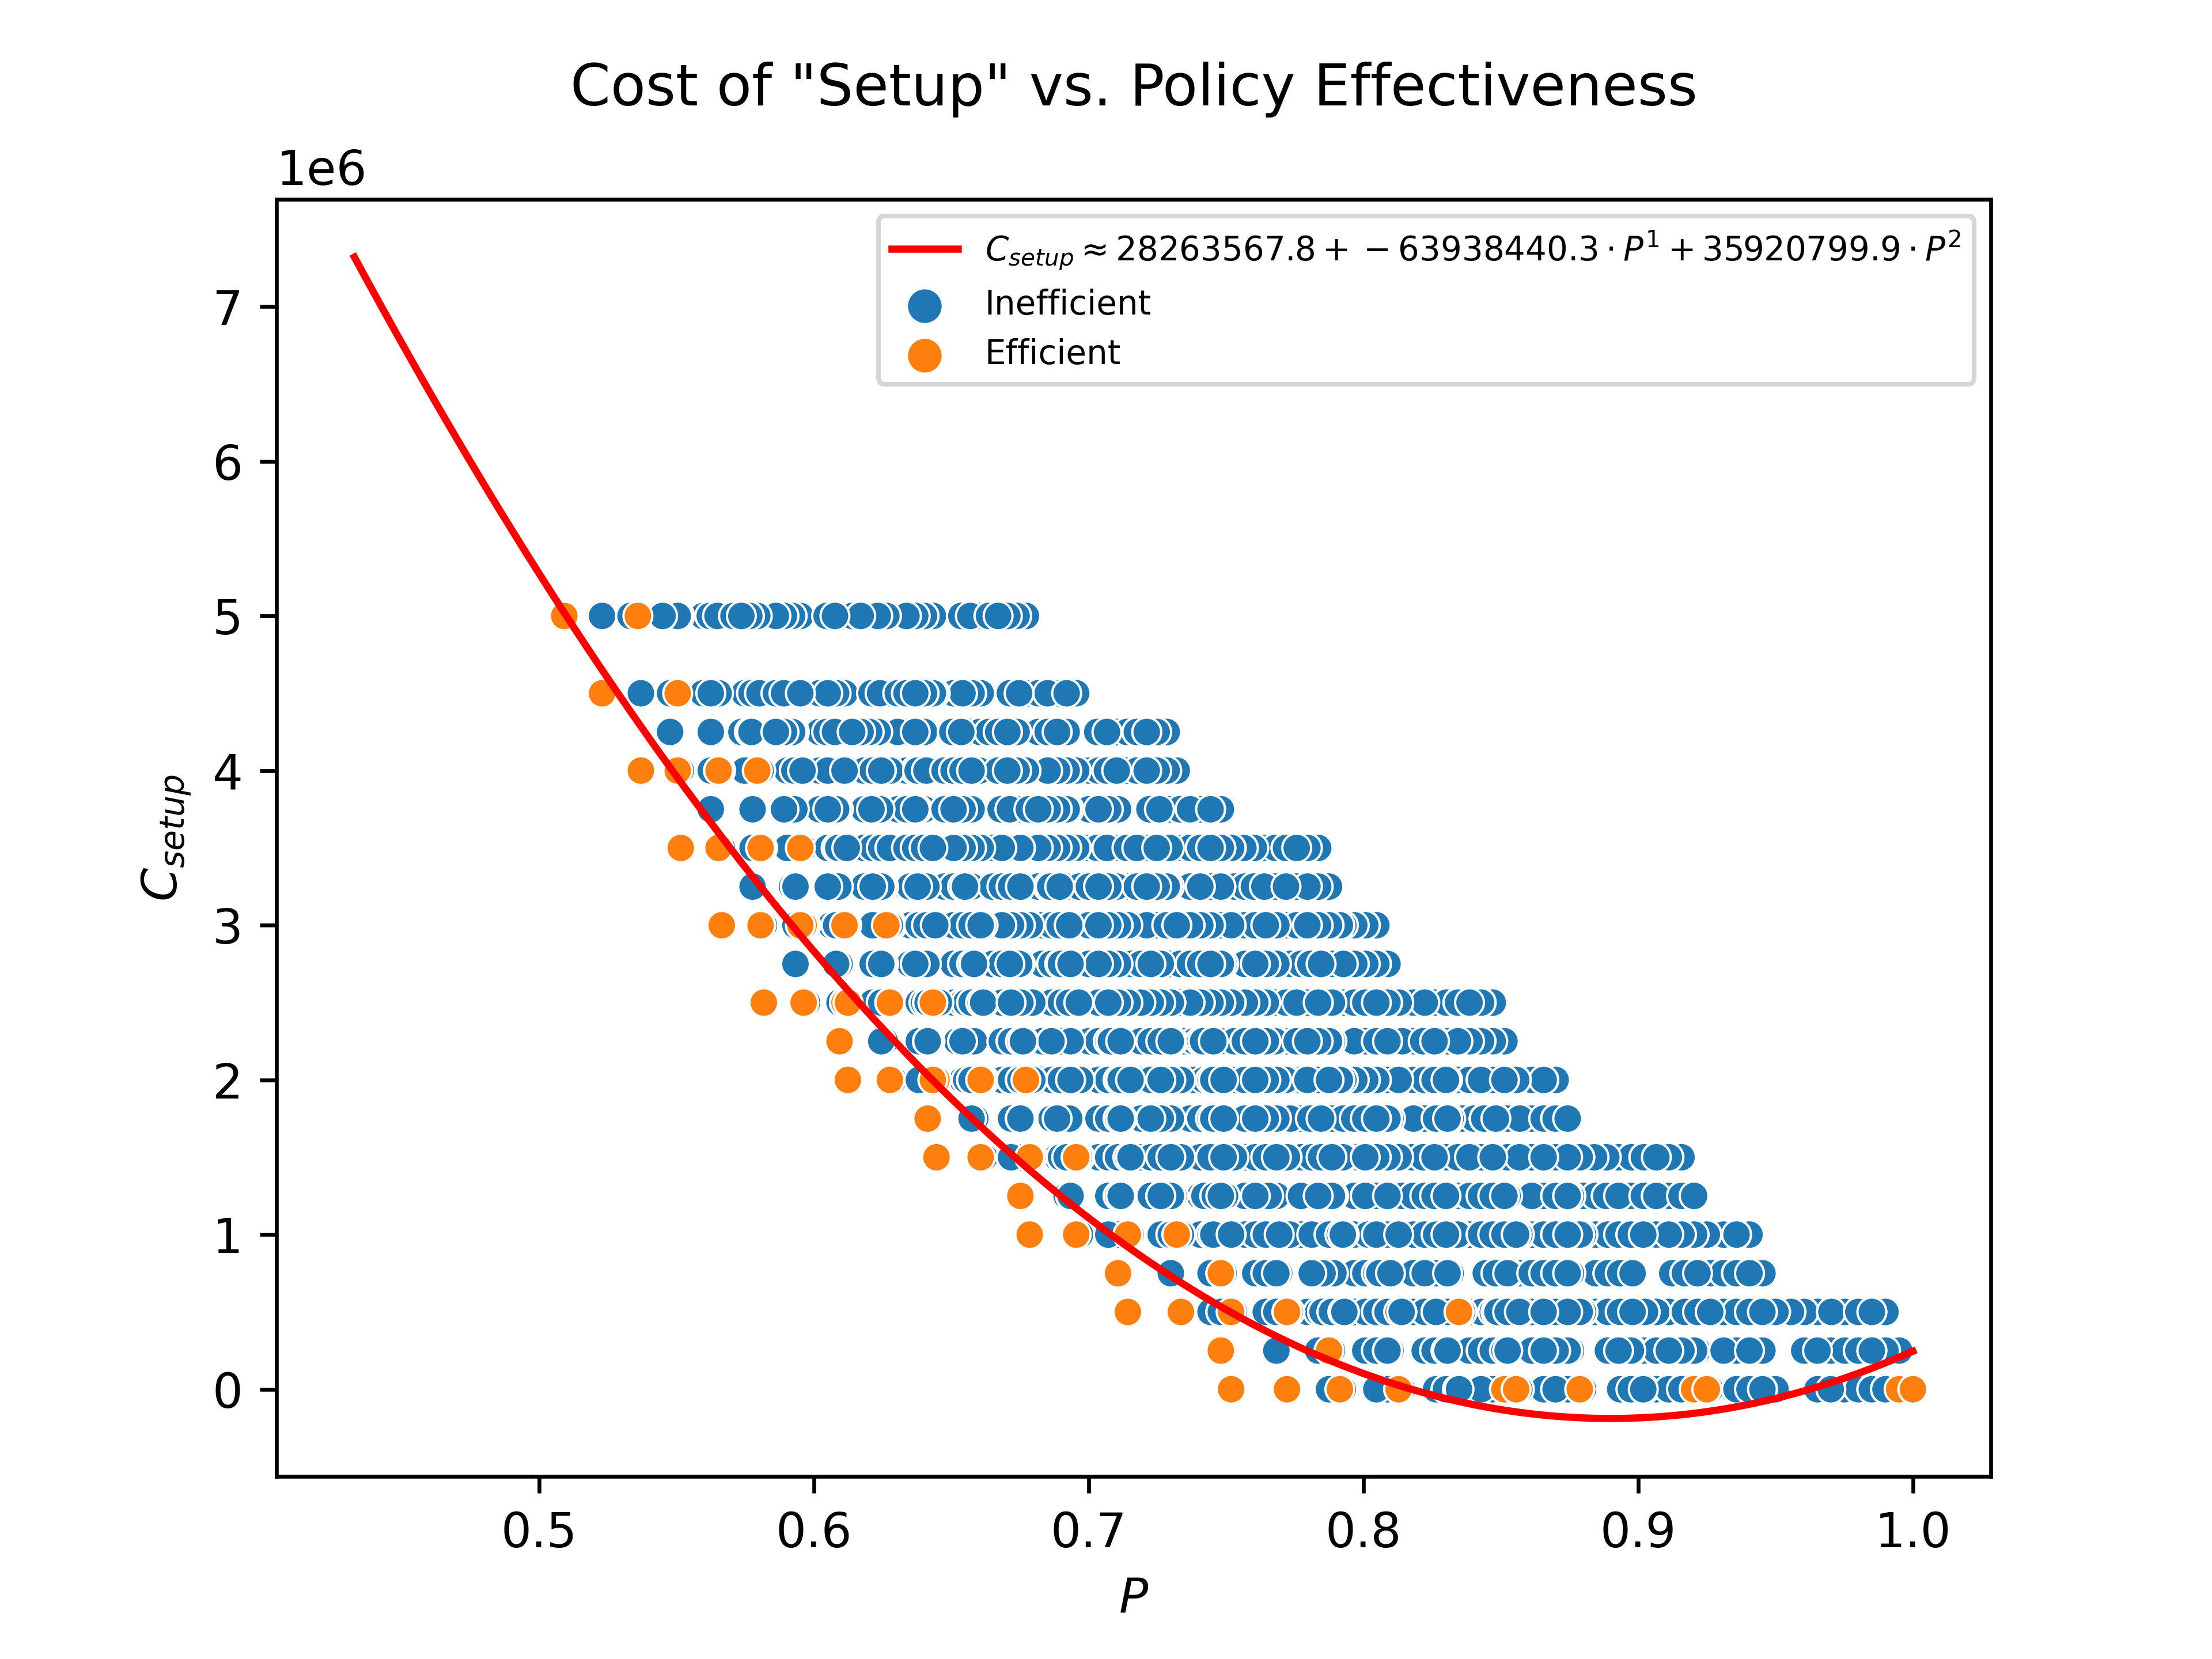
\includegraphics[width=0.46\linewidth]{figures/efficient_policies_setup.png}
    % 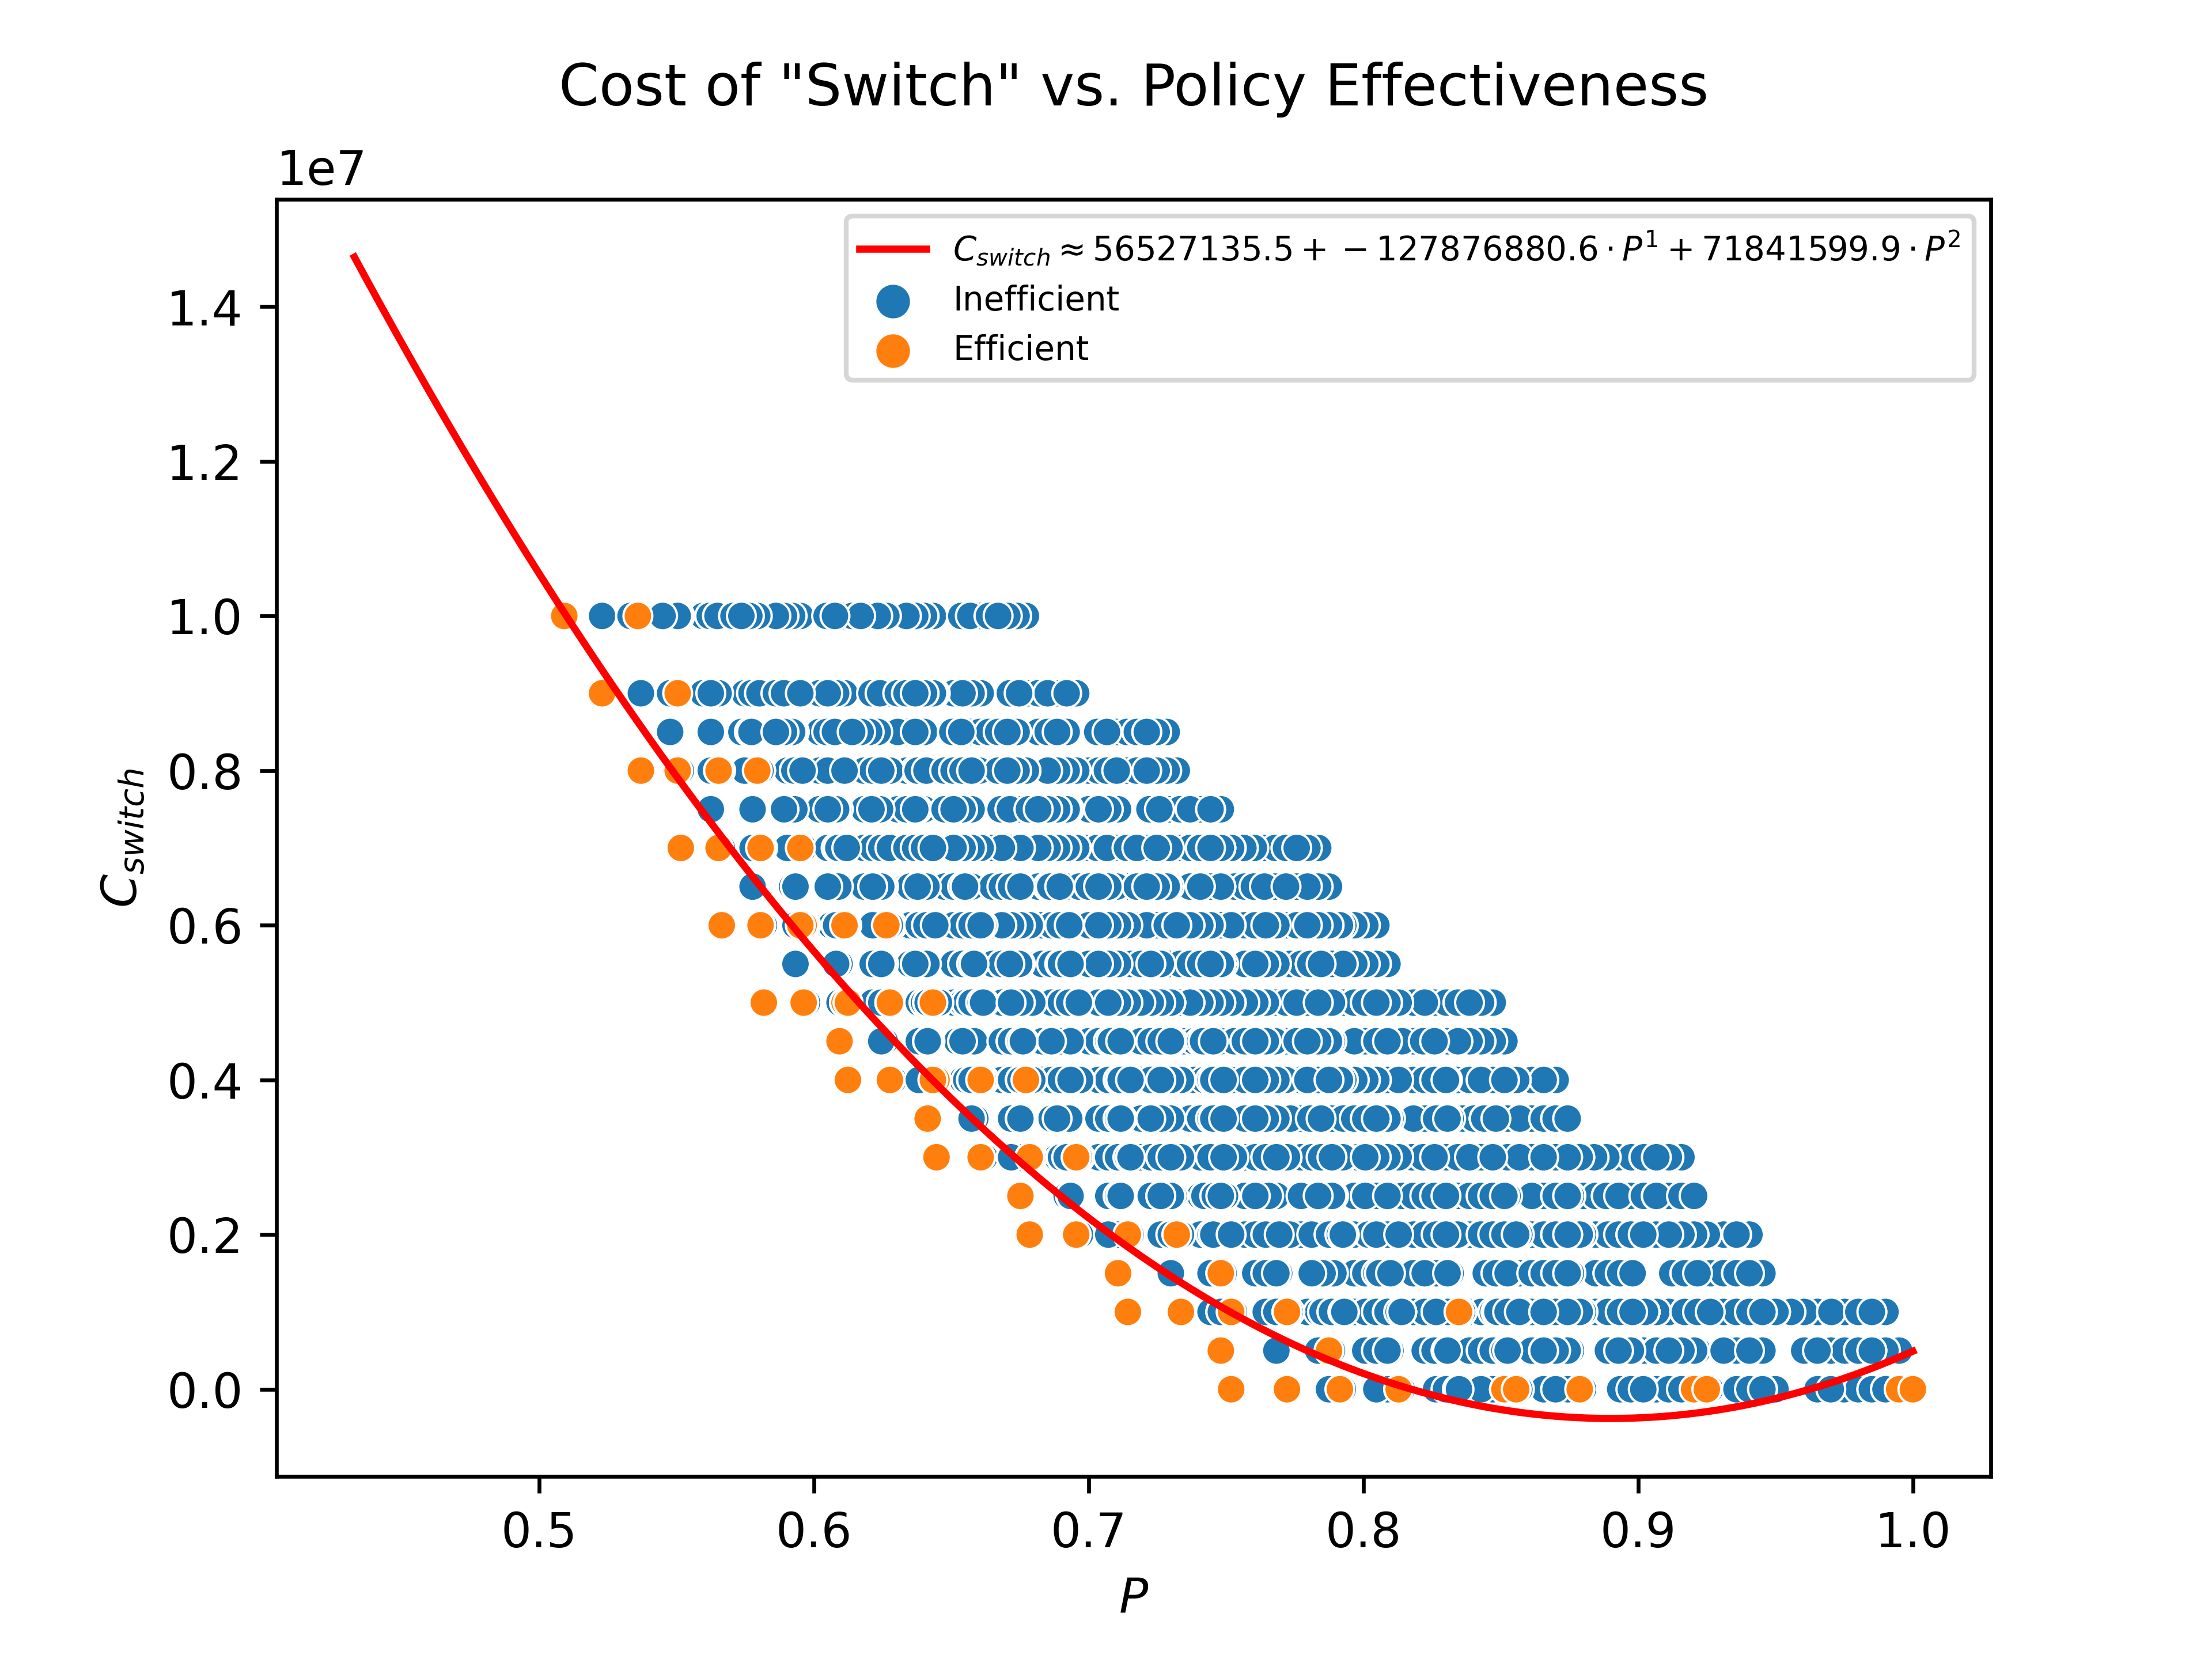
\includegraphics[width=0.46\linewidth]{figures/efficient_policies_switch.png}
    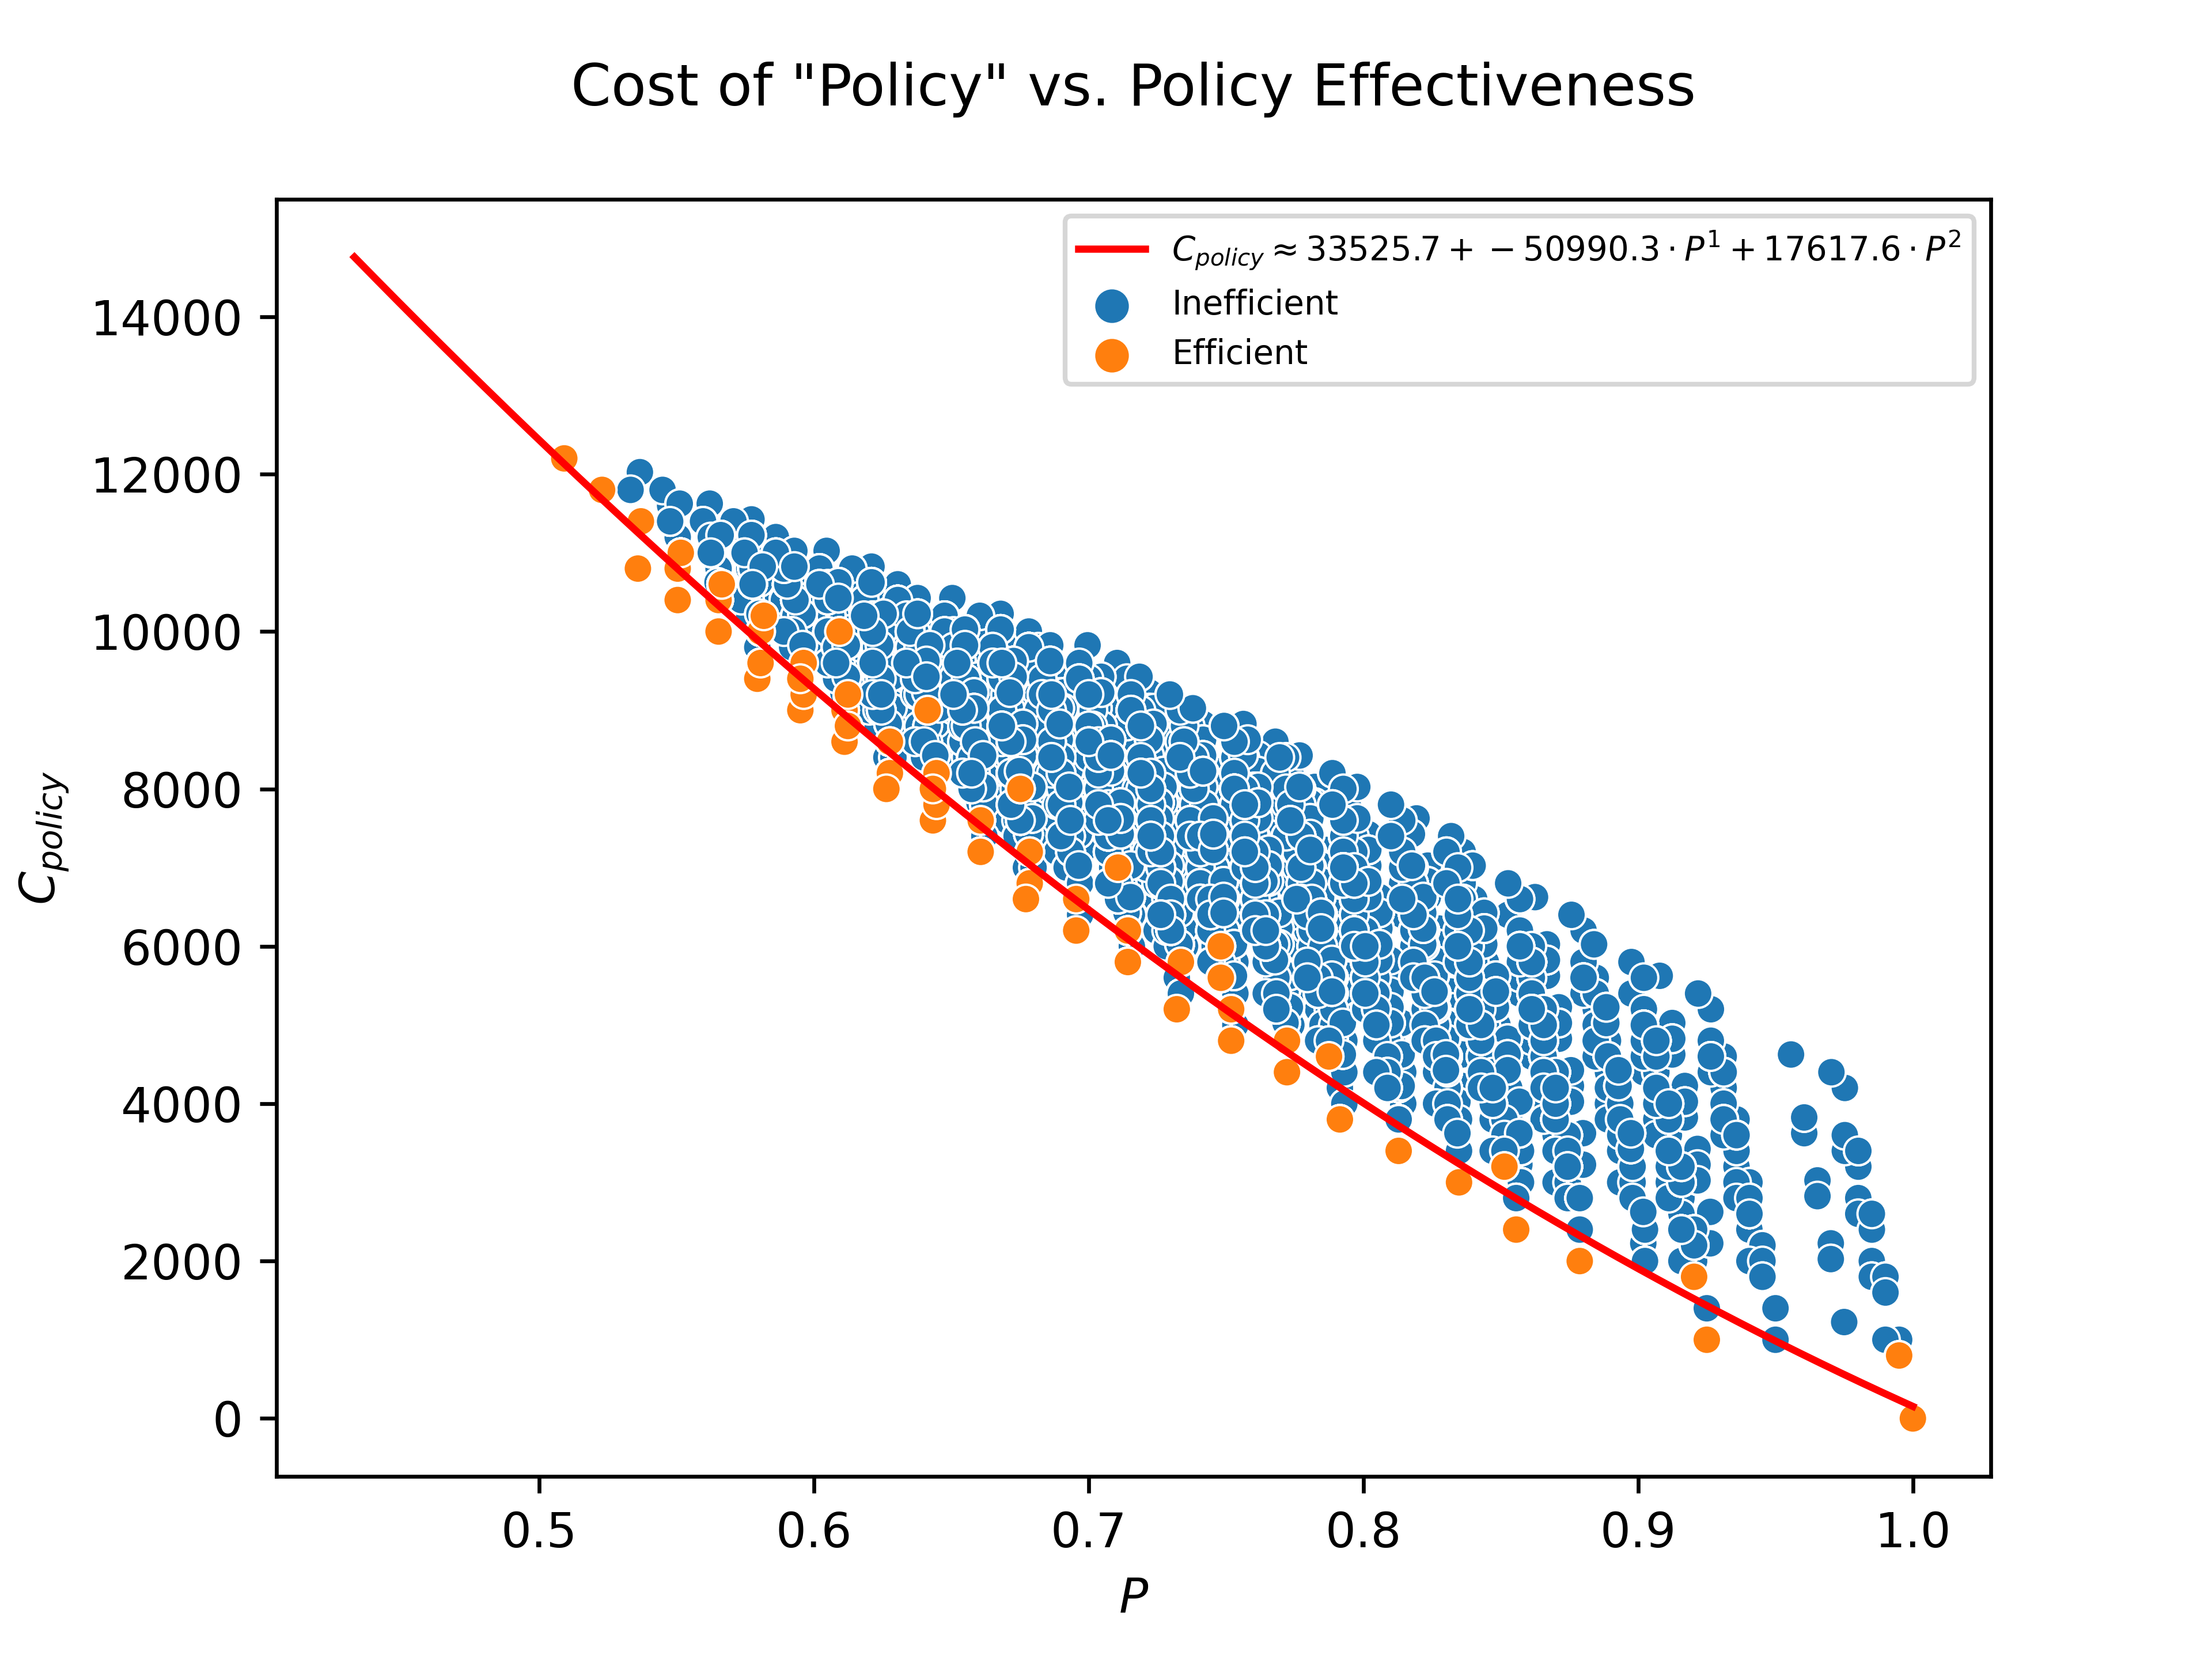
\includegraphics[width=0.46\linewidth]{figures/efficient_policies_policy.png}
    \caption{From all possible assortments of the policies listed in Section \ref{sec:params_table}, ``efficient'' assortments are approximated by a quadratic function of ``effectiveness'' $P_t$.}\label{fig:policy_approx}
\end{figure}

Given the $9$ atomic policies described in Section \ref{sec:params_table}, each with between $1$ and $4$ levels, there are a total of $51,840$ possible policy assortments. Remarkably, only $61$ of these assortments are non-dominated. For example, one of the ``efficient'' assortments in Figure \ref{fig:policy_approx} is ``Movement (level 1/2) \& Masking (level 2/3) \& Physical Distancing (level 1/1)'' parameters.

The \model problem can in fact be solved as a bilinear program (rather than a nonlinear program including higher-order terms) by considering policy assortments as the unit of analysis, rather than atomic policies. Unfortunately, even when restricting to ``efficient'' assortments, this does not yield a significantly more tractable problem, as there are still likely to be a relatively high number of possible assortments and a long time horizon. However, a quadratic approximation of policy assortments may be tractable and may yield interpretable high-level output.

Suppose, as in Figure \ref{fig:policy_approx}, the policy effectiveness of each assortment is calculated, and the setup and per-susceptible-individual costs of utilizing each assortment $\omega$ in period $t$ are approximated as follows:
\begin{itemize}
    \item If assortment $\omega$ is used in period $t$, then the policy effectiveness in the period is
    \begin{equation}\label{eq:assortment_P}
        P_t = P^\omega = \prod_{\substack{\{(i,j) : \text{policy $i$,}\\\text{level $j$ in $\omega$}\}}}P_{ijt}.
    \end{equation}

    There is a ``maximally effective'' policy assortment consisting of every atomic policy at the highest possible level. This assortment is always non-dominated, and its effectiveness $p_{min}$ serves as a lower bound for policy effectiveness: $p_{min} \le P_t \le 1$


   \item If assortment $\omega$ is used in period $t$, then the setup cost in the period is
    \begin{equation}\label{eq:assortment_A}
        A_t = A^\omega = \sum_{\substack{\{(i,j) : \text{policy $i$,}\\\text{level $j$ in $\omega$}\}}}A_{ijt}
    \end{equation}
    which we approximate as as ``$A(P_t)$'':
    \[
        A_t \approx a_2 P_t^2 + a_1 P_t + a_0
    \]

    \item If assortment $\omega$ is used in period $t$, then the per-susceptible-individual cost in the period is
    \begin{equation}\label{eq:assortment_C}
        C_t = C^\omega =  \sum_{\substack{\{(i,j) : \text{policy $i$,}\\\text{level $j$ in $\omega$}\}}}C_{ijt}
    \end{equation}
    which we approximate as ``$C(P_t)$'':
    \[
        C_t \approx c_2 P_t^2 + c_1 P_t + c_0
    \]
\end{itemize}

% \prod_{\substack{i,j \text{ s.t.}\\\text{policy $i$ used}\\\text{at level $j$}\\\text{in period $t$}}}

The following mathematical program describes this approximation (note the absence of switching costs):

{\small
    \begin{alignat}{4}
        &\Minimize_{P,A,C,S,I,R,D,d}\qquad \span\span\span\span\sum_{t=1}^{T}A_t + C_{t} S_{t}  + \sum_{t=1}^{T}C_{infection} I_t &&+ C_{death}  d_t \label{eq:quadratic_approx}\\
        & \text{s.t.}\qquad  && S_t &&= S_{t-1} - K_I \cdot P_t \cdot S_{t-1} \cdot I_{t-1} && \fa t \in \{2,\ldots,T\} \nonumber\\
        & {} && I_t &&= I_{t-1} + K_I \cdot P_t \cdot S_{t-1} \cdot I_{t-1} - K_R\cdot I_{t-1} - K_D \cdot I_{t-1} && \fa t \in \{2,\ldots,T\} \nonumber\\
        & {} && R_t &&= R_{t-1} + K_R \cdot I_{t-1} && \fa t \in \{2,\ldots,T\} \nonumber\\
        & {} && d_t &&= K_D \cdot I_{t-1} && \fa t \in \{2,\ldots,T\} \nonumber\\
        & {} && D_t &&= D_{t-1} + d_t && \fa t \in \{2,\ldots,T\} \nonumber\\
        & {} && A_t &&=  a_2 P_t^2 + a_1 P_t + a_0&& \fa t \in \{1,\ldots,T\} \nonumber\\
        & {} && C_t &&= c_2 P_t^2 + c_1 P_t + c_0&& \fa t \in \{1,\ldots,T\} \nonumber\\
        & {} && p_{min} &&\le P_t \le 1&& \fa t \in \{1,\ldots,T\} \nonumber\\
        & {} && I_1 &&= I_0 && \nonumber\\
        & {} && S_1 &&= N - I_0 && \nonumber\\
        & {} && D_1 &&= 0 && \nonumber\\
        & {} && R_1 &&= 0 && \nonumber\\
        & {} && d_1 &&= 0 && \nonumber
    \end{alignat}
}

A solution to problem \eqref{eq:quadratic_approx} yields a natural heuristic solution method for the \model mode \eqref{eq:objective0} by finding policy assortments that yield similar cost and probability decisions. Specifically, for any value of $(A_t, C_t, P_t)$, let $\omega(A_t,C_t,P_t)$ be the policy assortment that yields the ``closest'' values $(A^\omega, C^\omega, P^\omega)$ as defined by equations \eqref{eq:assortment_P}, \eqref{eq:assortment_A}, and \eqref{eq:assortment_C} and some loss function $L$. Consider the loss function
\begin{equation}\label{eq:assortment_loss_function}
    L((A,C,P),\omega) =(P^\omega-P)^2
\end{equation}
and then the ``closest'' policy is defined as
\begin{equation}\label{eq:assortment_loss_minimizer}
    \omega(A,C,P) = \argmin_{\omega\in \Omega} L((A,C,P),\omega).
\end{equation}
Finally, recalling that $j_{\omega i}$ is the level of policy $i$ implied by assortment $\omega$, define the mapping of a policy assortment $\omega$ to a binary decision of whether intervention $i$ is used at level $j$ as:
\begin{equation}
    y_{ij}^{\omega} = \begin{cases}1 &: j=j_{\omega i}\\ 0 &: \text{otherwise}\end{cases}.
\end{equation}

The heuristic solution method utilizing solutions of the quadratically approximated problem \eqref{eq:quadratic_approx} can then be written as follows:
\begin{pseudocode}
    Solve approximated problem |\eqref{eq:quadratic_approx}| to obtain |$A_t, C_t, P_t$| for all t.
    Calculate the ``closest'' assortment for each period |$\omega_t = \omega(A_t,C_t,P_t)$|
    Use the policy decisions in the full |\model| problem by substituting |$y_{ijt}=y^{\omega_t}_{ij}$|
\end{pseudocode}


\section{Results}

\subsection{Comparison of Heuristics}\label{sec:comparison_of_heuristics}

Here we present three solutions for the same \model instance with $T=100$ periods, calculated using different heuristics. The first is the ``$F$-Factor Early Stopping'' heuristic defined in Section \ref{sec:early_stopping} with $F=0.8$; the second is the Lagrangian heuristic defined in Section \ref{sec:lagrangian}; the third is the quadratic heuristic defined in Section \ref{sec:quadratic_approximation}.

Note that the early-stopping heuristic in Figure \ref{fig:heuristic_early_stopping} generates the best solution overall, the Lagrangian solution in Figure \ref{fig:heuristic_lagrangian}, utilizing the Lagrangian lower-bound, has the tightest lower-bound\footnote{the listed lower bound of the quadratic approximation is not a true lower bound, but a lower bound of the quadratic approximation \eqref{eq:quadratic_approx}}, and the quadratic approximation in Figure \ref{fig:heuristic_quadratic}, which is solved by ignoring switching costs, has the most policy changes over the horizon.

\begin{figure}[H]
    \begin{subfigure}{\textwidth}
        \begin{center}
            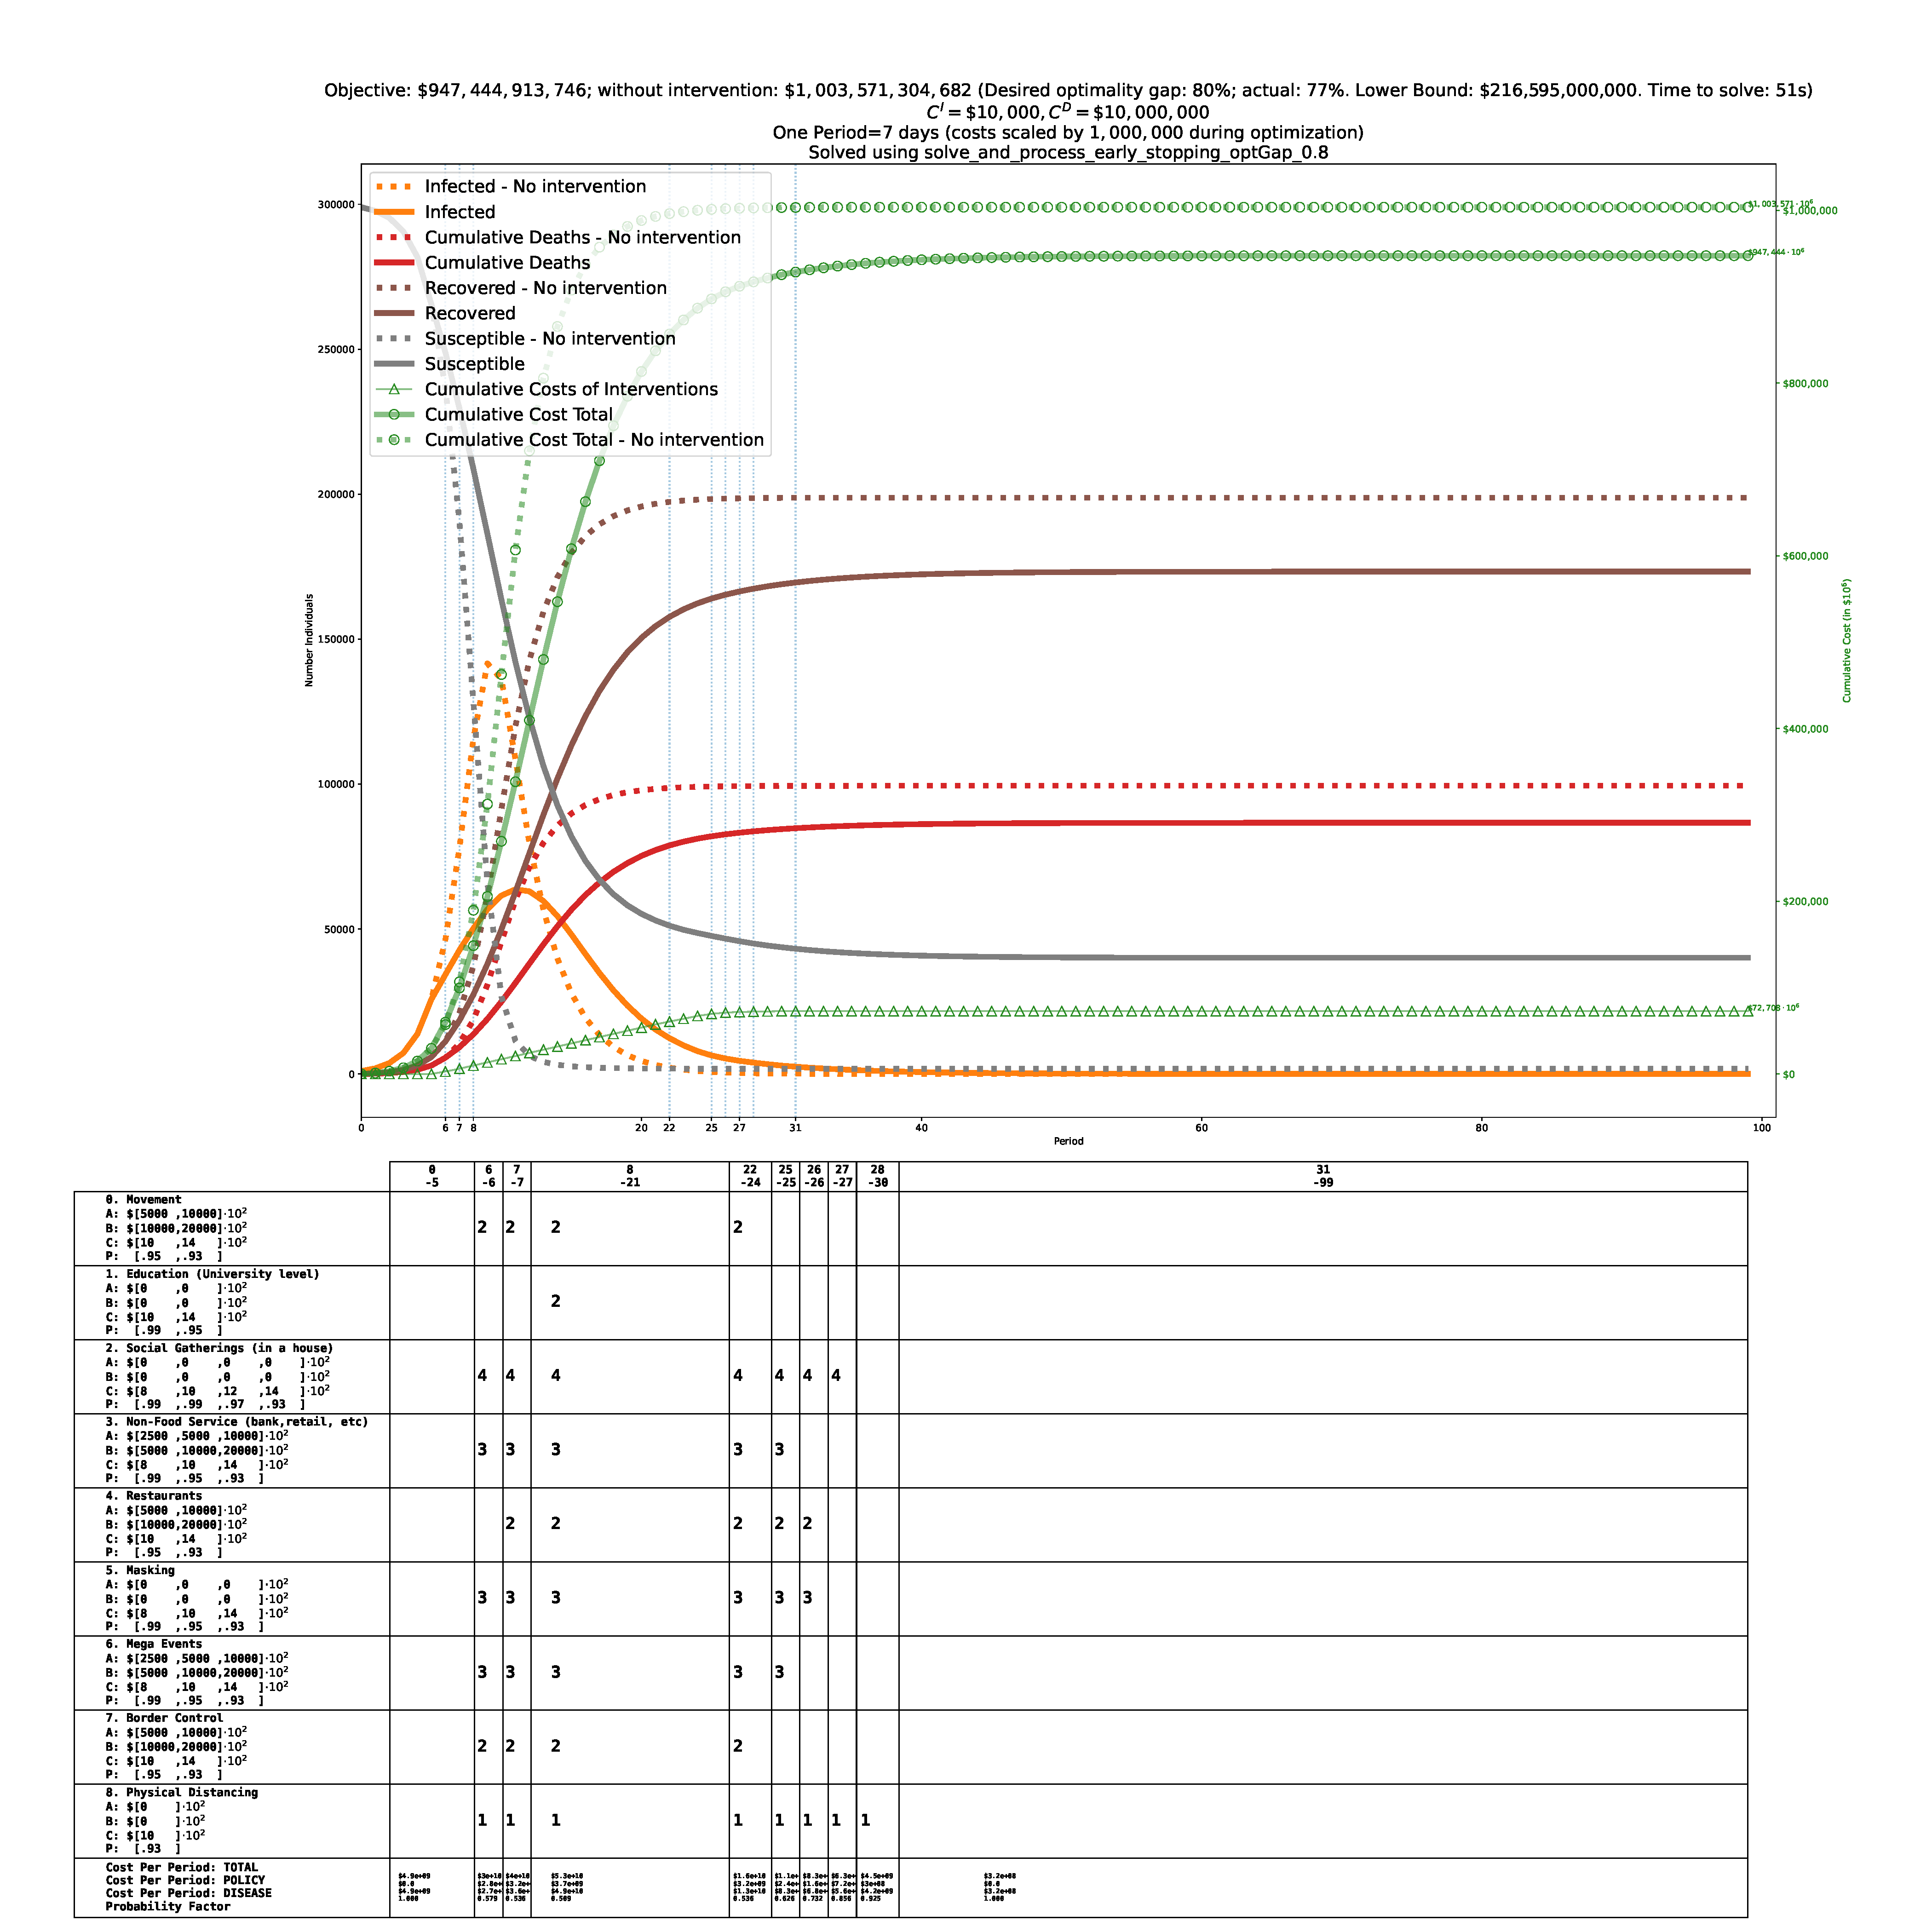
\includegraphics[width=1.2\linewidth]{figures/heuristic_solutions/system_state_vs_time_T100_baron__solve_and_process_early_stopping_optGap_0.8.pdf}
        \end{center}
        \caption{Solution using $0.8$-Factor Early Stopping heuristic with the BARON solver.}\label{fig:heuristic_early_stopping}
    \end{subfigure}
\end{figure}

\begin{figure}[H]\ContinuedFloat
    \begin{subfigure}{\textwidth}
        \begin{center}
            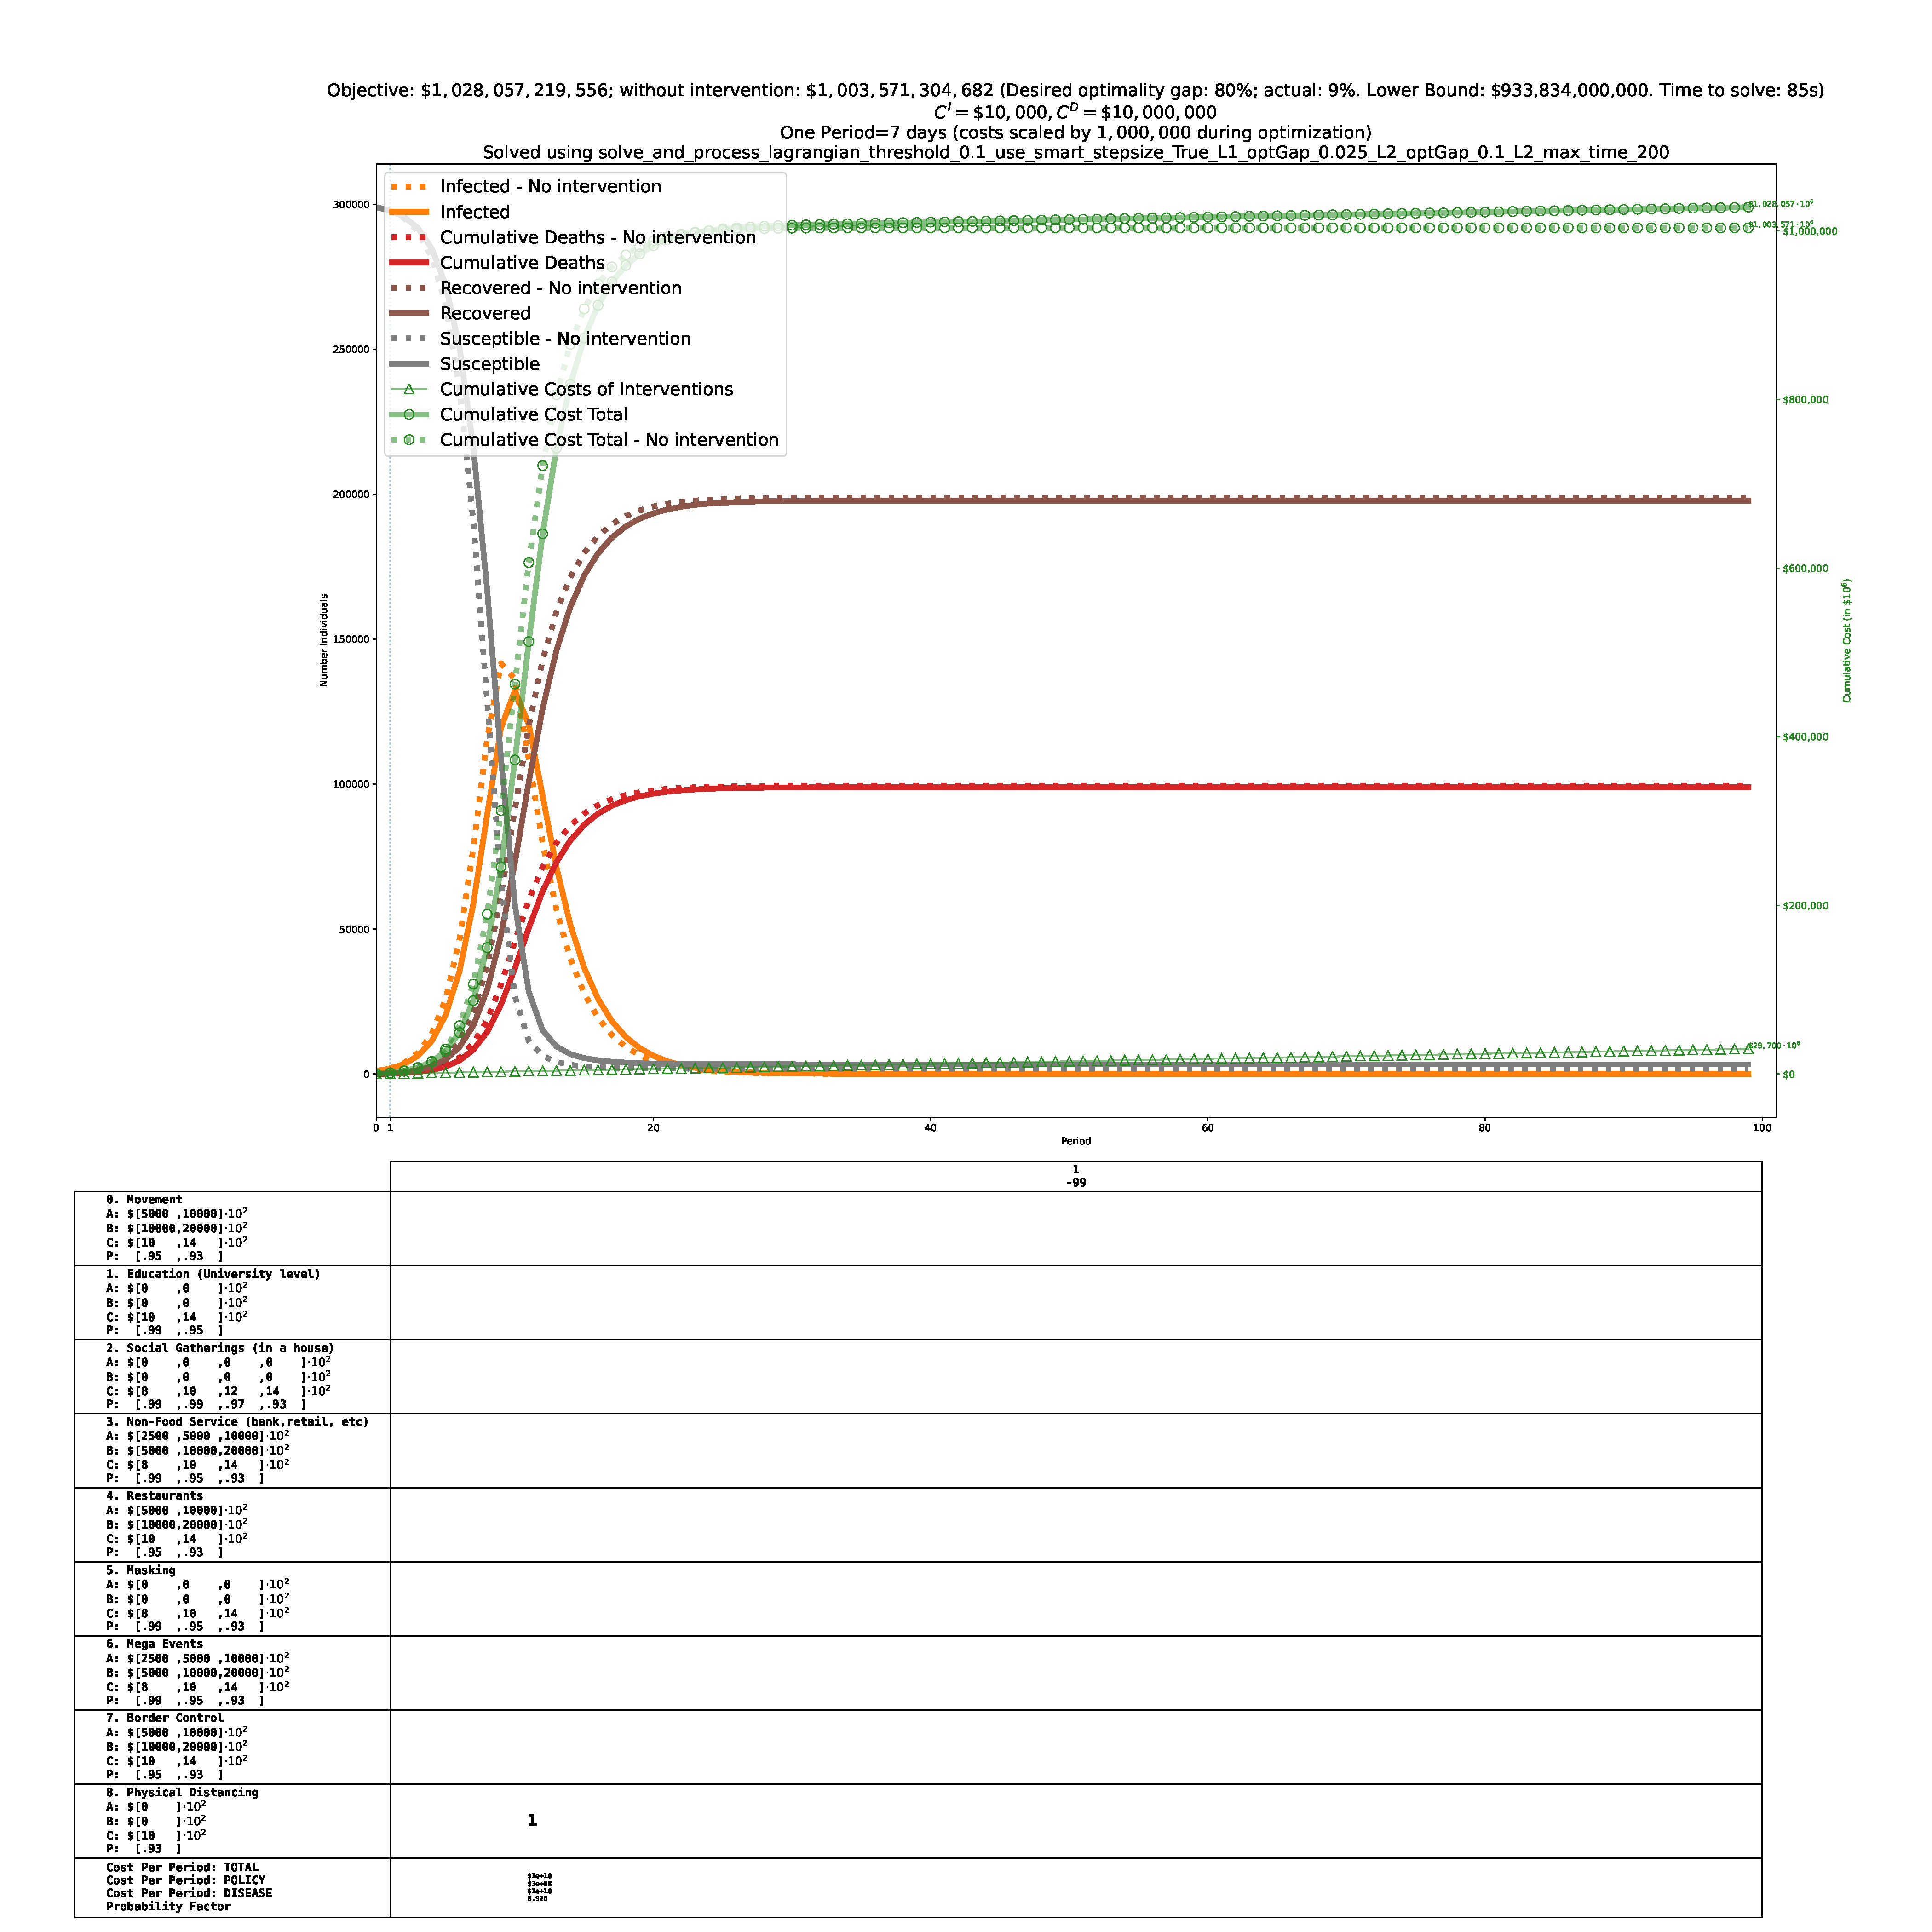
\includegraphics[width=1.2\linewidth]{figures/heuristic_solutions/system_state_vs_time_T100_baron__solve_and_process_lagrangian_threshold_0.1_use_smart_stepsize_True_L1_optGap_0.025_L2_optGap_0.1_L2_max_time_200.pdf}
        \end{center}
        \caption{Solution using the Lagrangian heuristic.}\label{fig:heuristic_lagrangian}
    \end{subfigure}
\end{figure}

\begin{figure}[H]\ContinuedFloat
    \begin{subfigure}{\textwidth}
        \begin{center}
            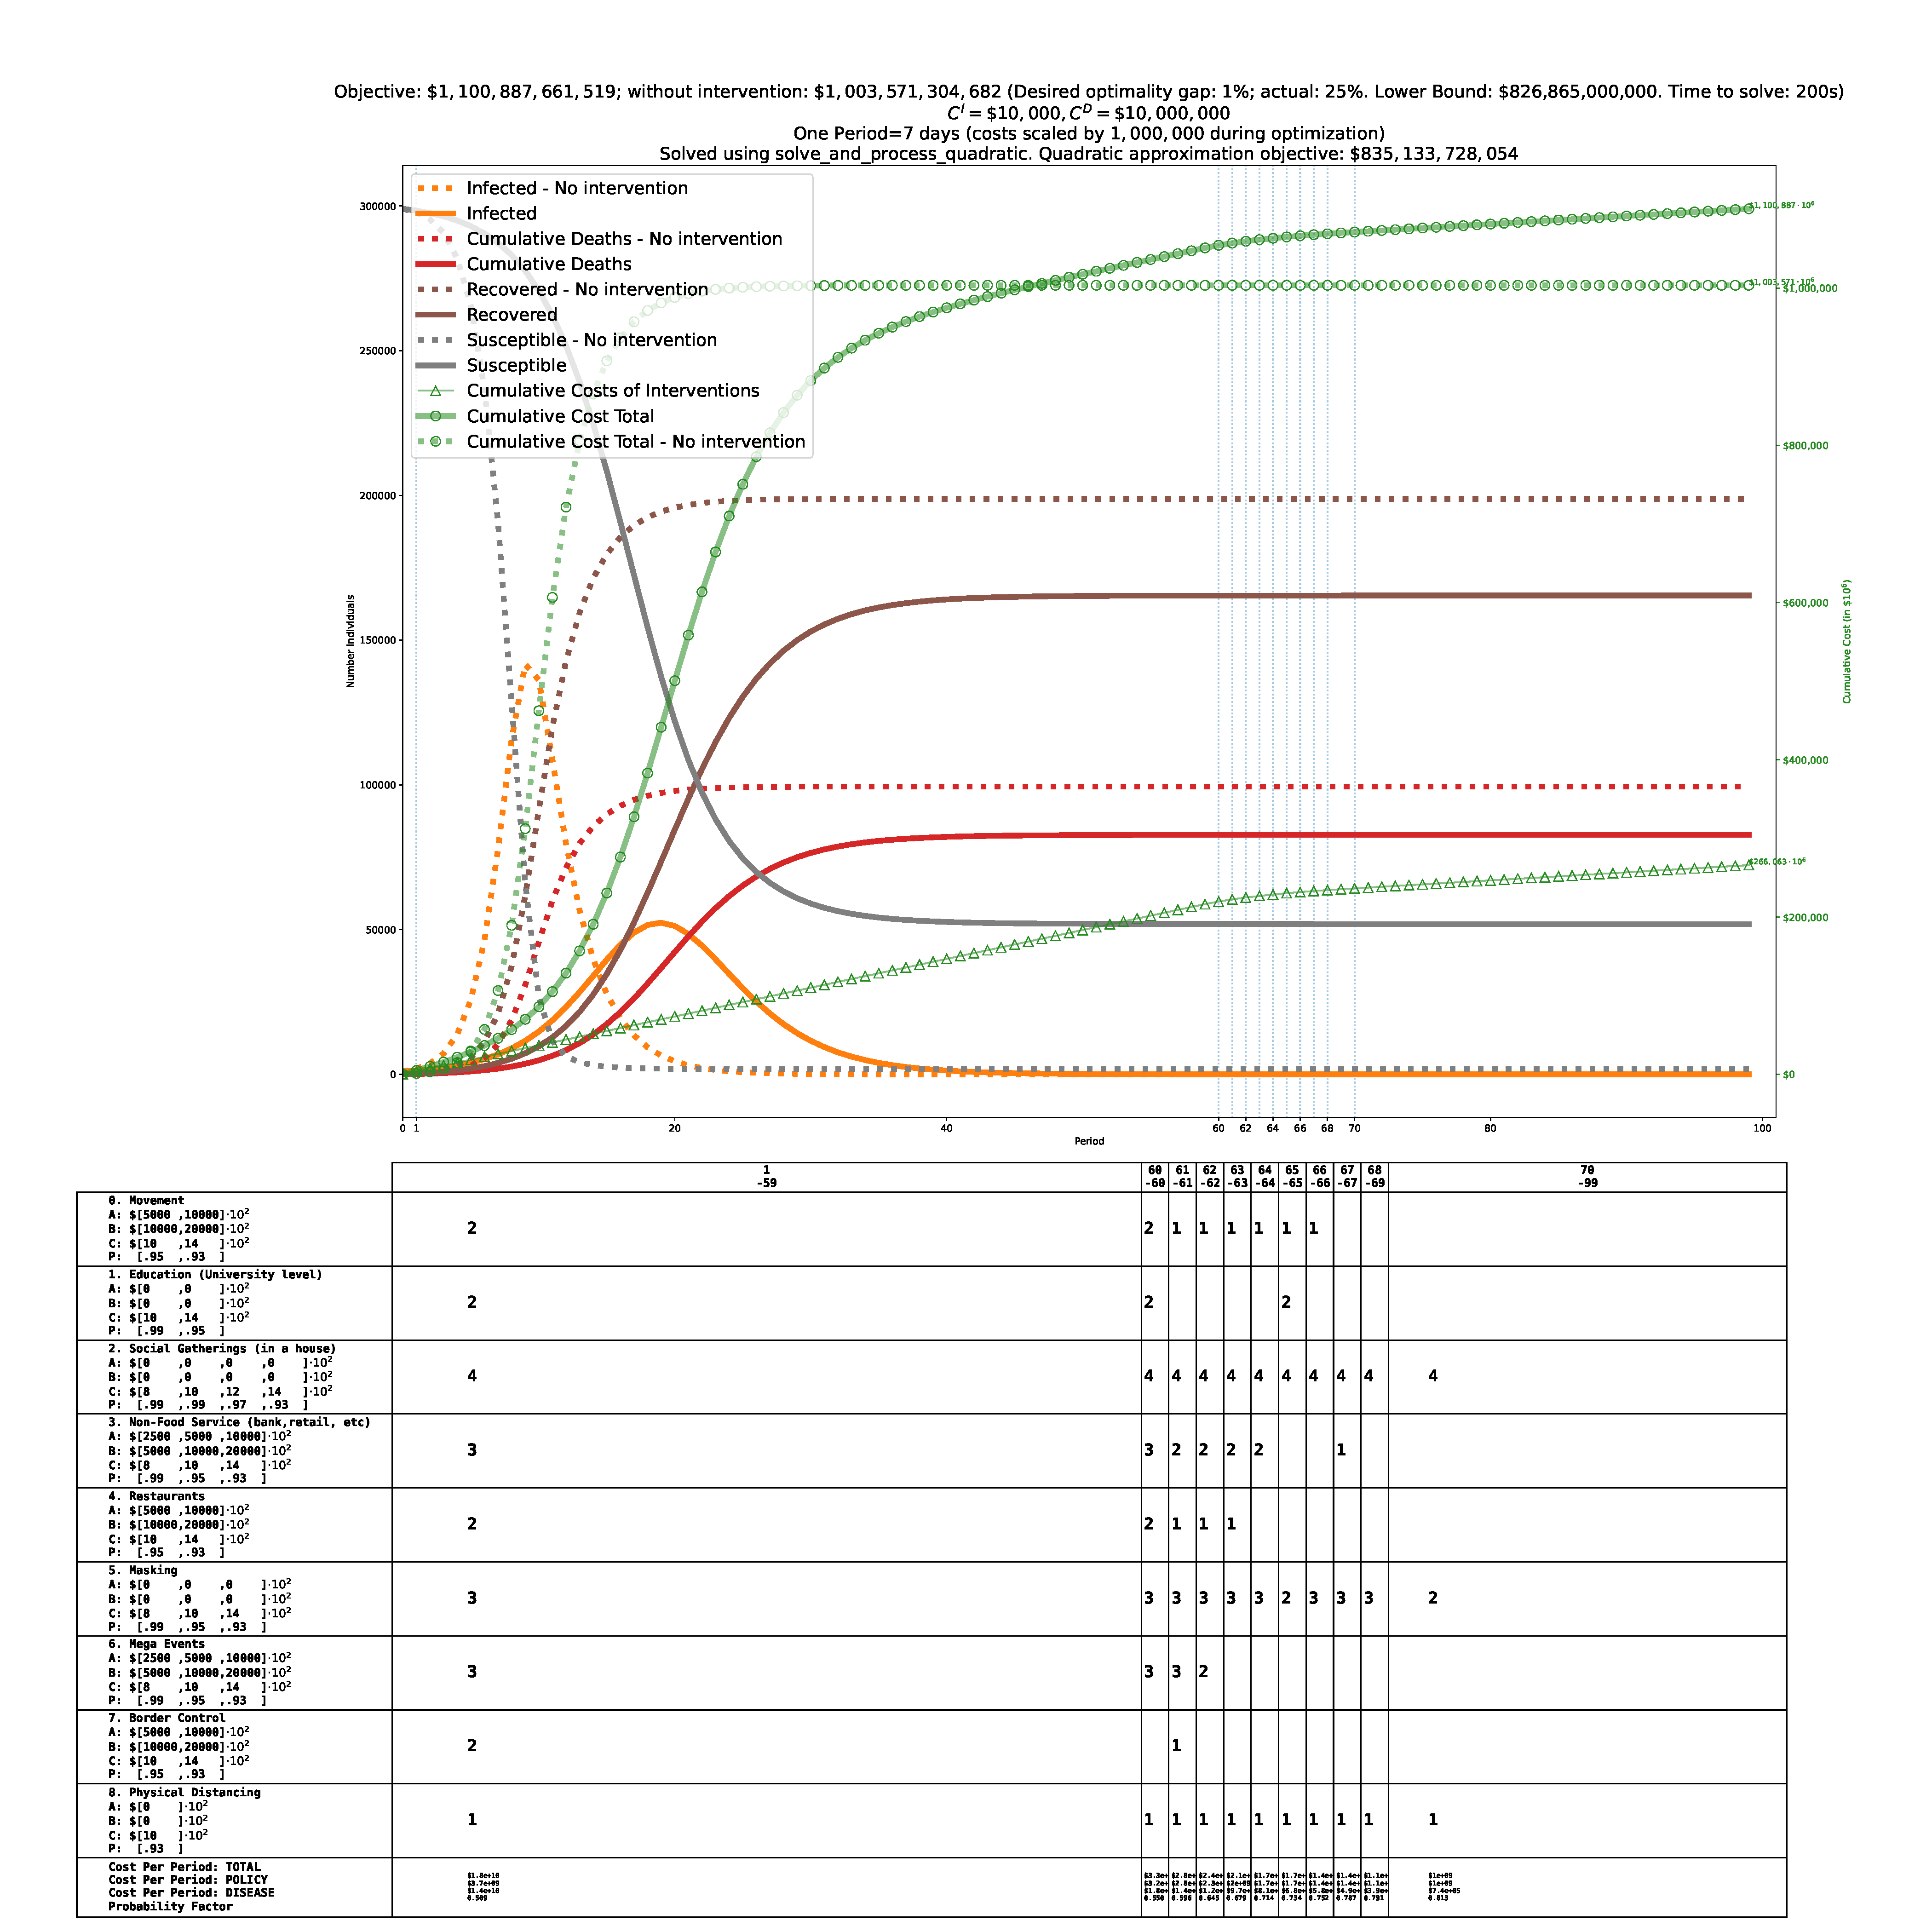
\includegraphics[width=1.2\linewidth]{figures/heuristic_solutions/system_state_vs_time_T100_baron__solve_and_process_quadratic.pdf}
        \end{center}
        \caption{Solution using the quadratic approximation. Note that the lower bound listed is a lower bound on the quadratic approximation \eqref{eq:quadratic_approx}, not the full \model problem.}\label{fig:heuristic_quadratic}
    \end{subfigure}
\end{figure}

\begin{figure}[H]\ContinuedFloat
    \begin{subfigure}{\textwidth}
        \begin{center}
            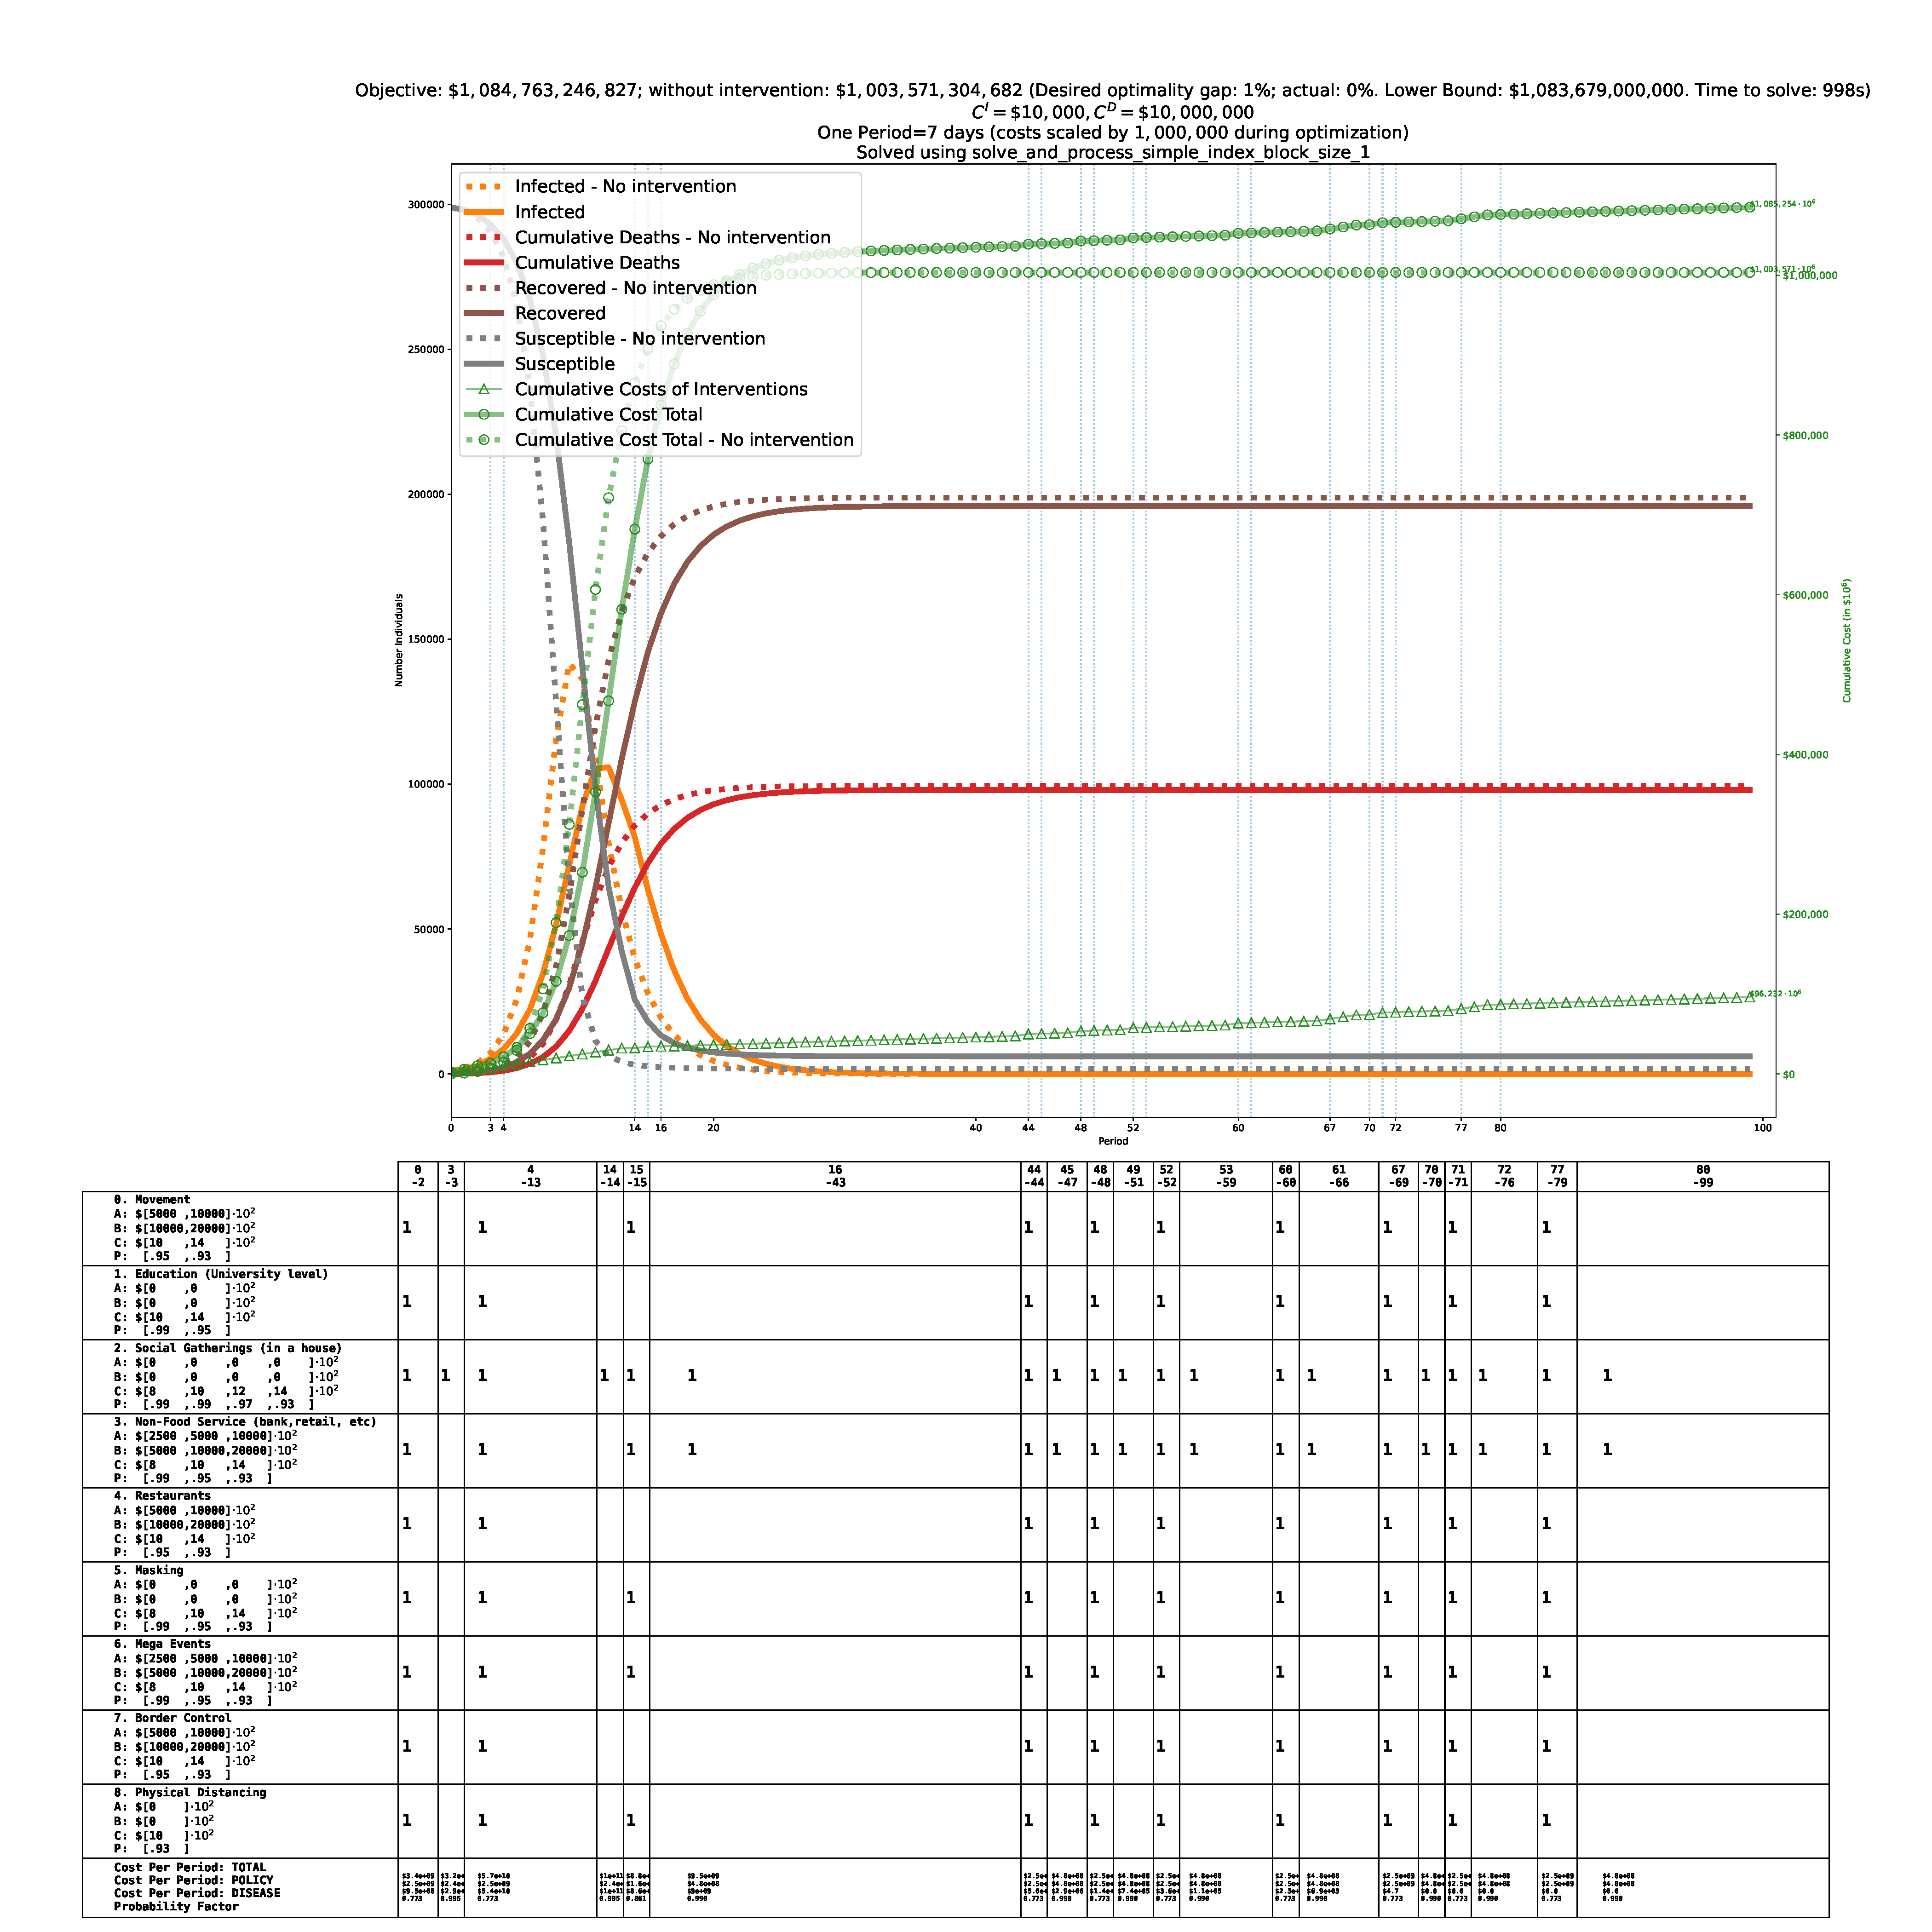
\includegraphics[width=1.2\linewidth]{figures/heuristic_solutions/system_state_vs_time_T100_baron__solve_and_process_simple_index_block_size_1.pdf}
        \end{center}
        \caption{Solution using the index policy described in Section \ref{sec:heuristic_index}, using a block size of $b=1$.}\label{fig:heuristic_index_blocksize1}
    \end{subfigure}
\end{figure}


\begin{figure}[H]\ContinuedFloat
    \begin{subfigure}{\textwidth}
        \begin{center}
            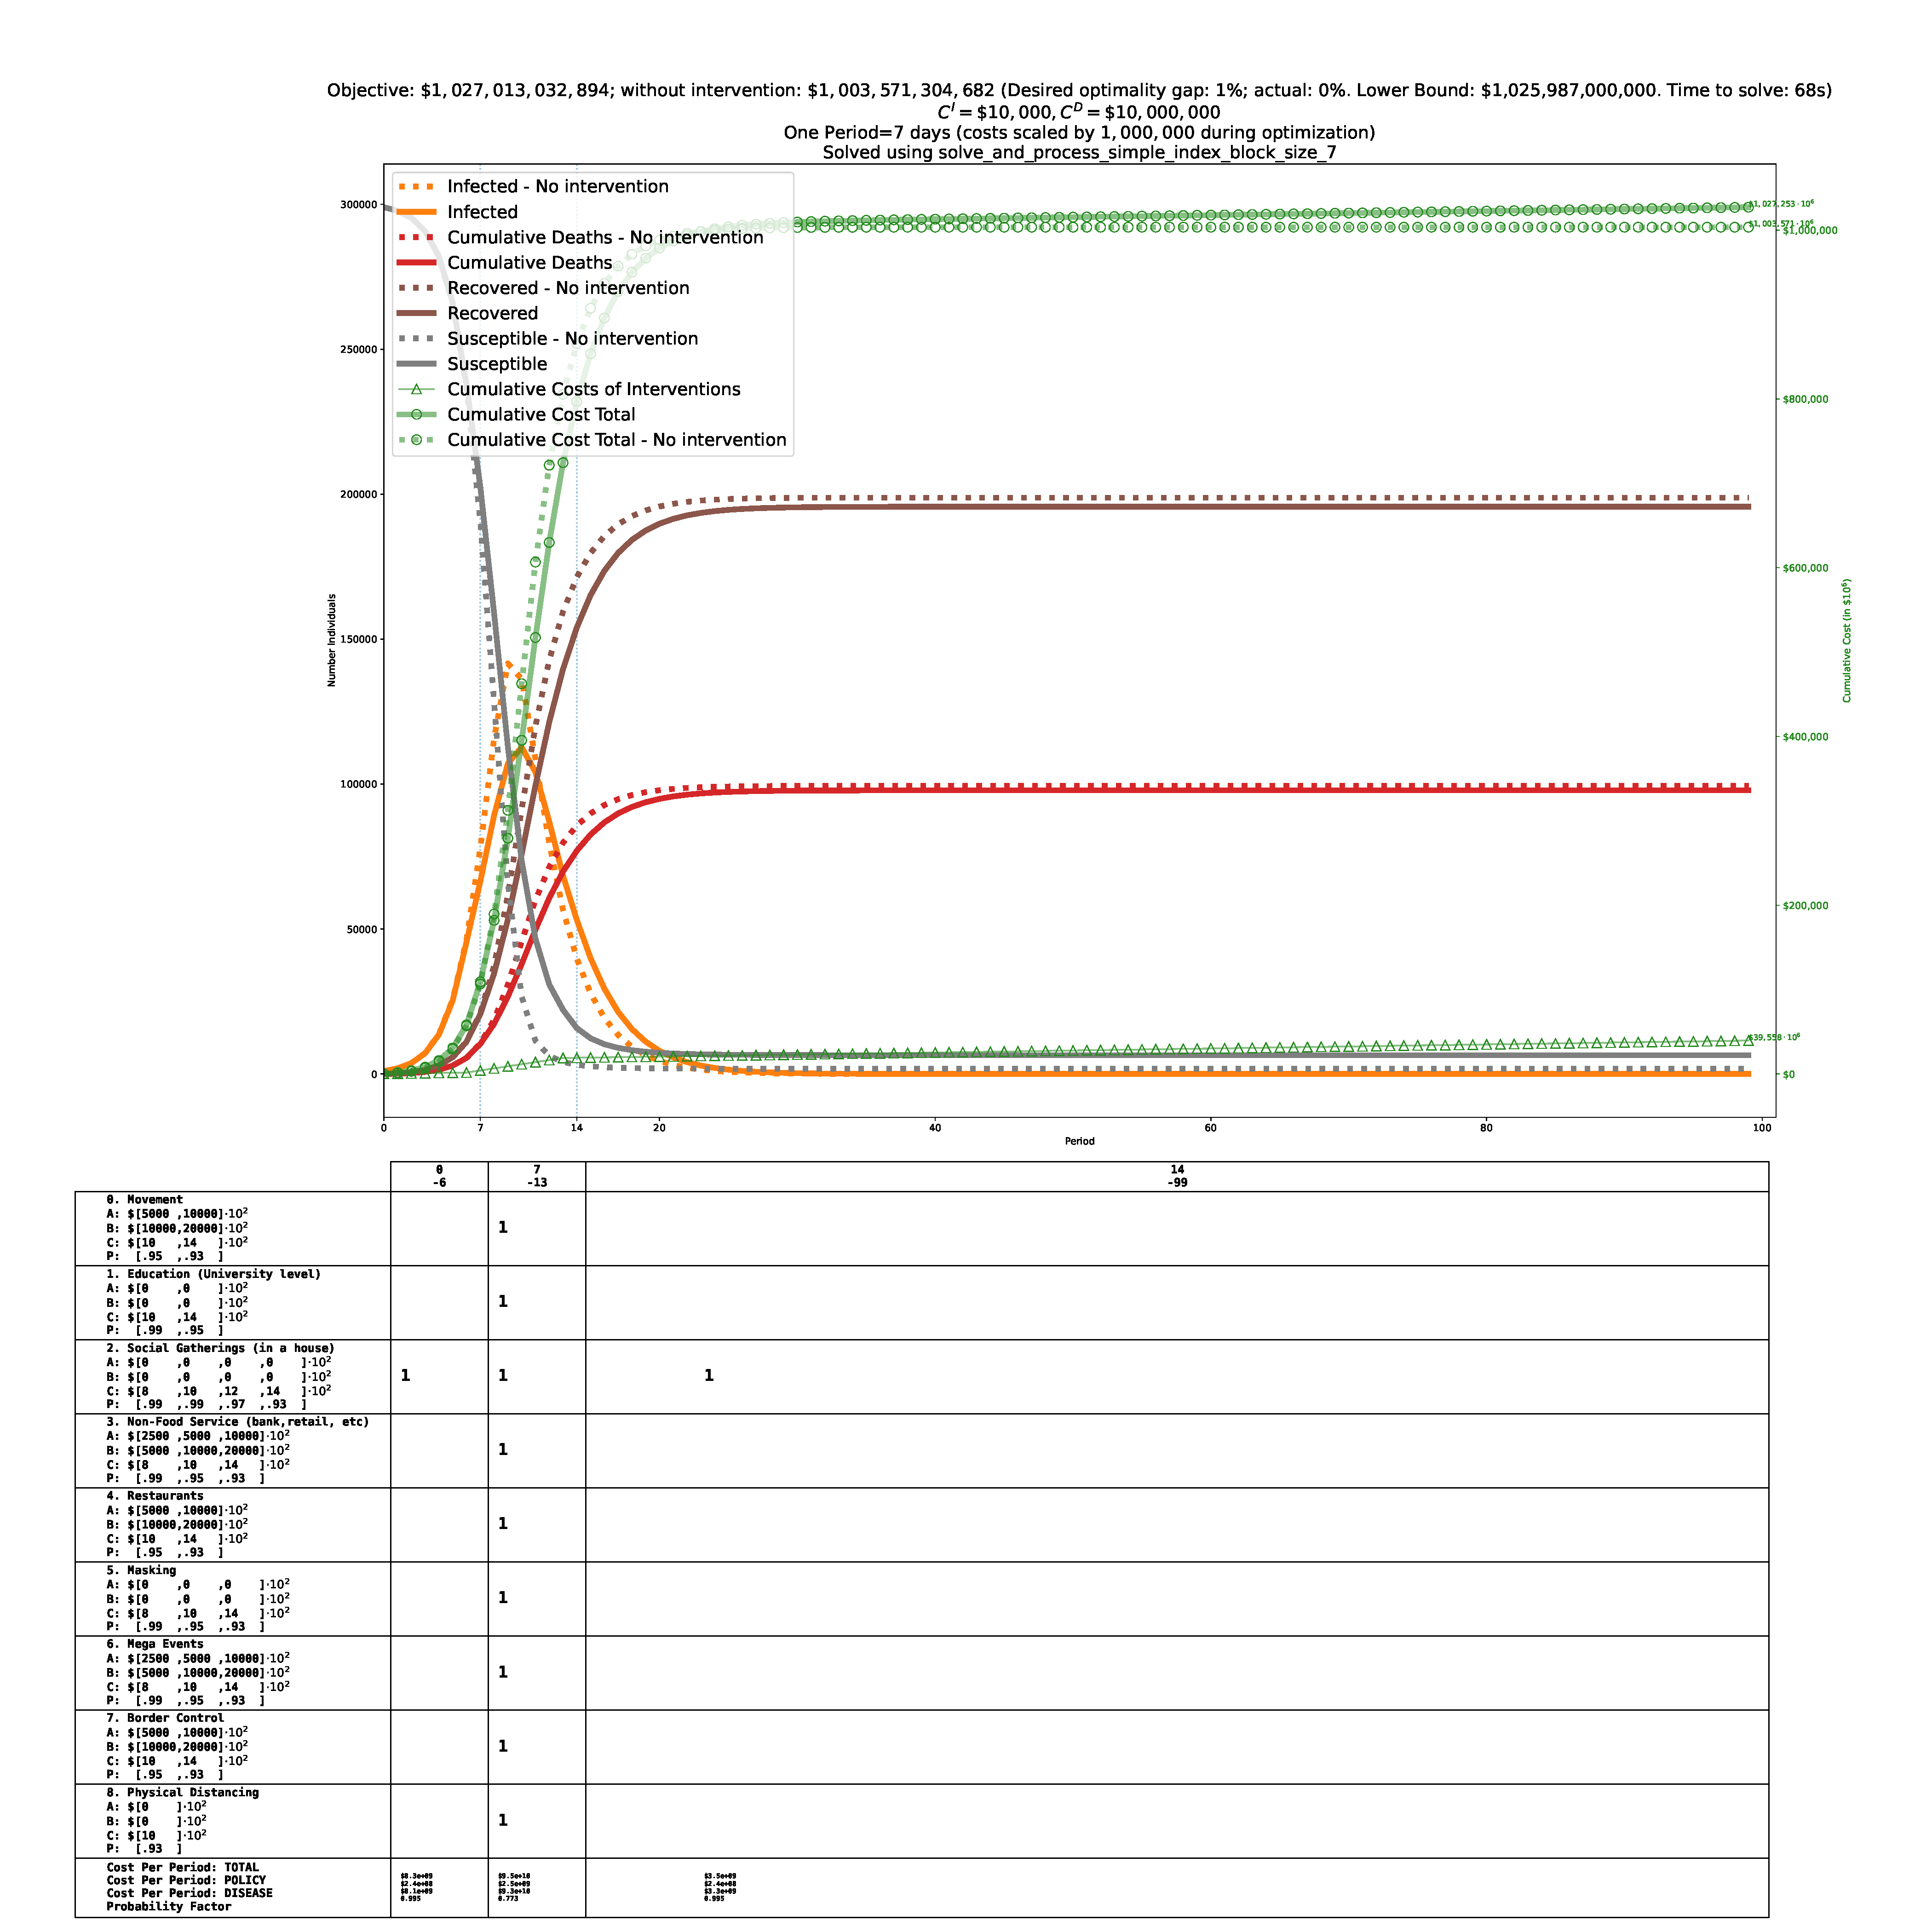
\includegraphics[width=1.2\linewidth]{figures/heuristic_solutions/system_state_vs_time_T100_baron__solve_and_process_simple_index_block_size_7.pdf}
        \end{center}
        \caption{Solution using the index policy described in Section \ref{sec:heuristic_index}, using a block size of $b=7$.}\label{fig:heuristic_index_blocksize7}
    \end{subfigure}
\end{figure}


\subsection{Lagrangian Heuristic Lower Bound Improvement}

The lower bound on the objective value of \model obtained by optimizing the (decomposed) Lagrangian relaxation described in Section \ref{sec:lagrangian} seems relatively tight on several problem instances. The corresponding heuristic also performs quite well. On the other hand, the BARON solver is able to generate solutions within a few minutes to the full \model problem that are extremely high quality, but it does not guarantee a reasonable level of optimality even after running for hours. In particular, the BARON solver generates lower bounds as part of its numerical optimization procedure, but these lower bounds are nowhere near the values it obtains. The bounds generated by the Lagrangian procedure prove that these solutions are nearly optimal. This yields a stopping condition for the BARON solver that guarantees a desired level of optimality.

The following trials were considered to evaluate the performance of the Lagrangian method:

\input{lagrangian_table_figure.tex}


\subsubsection{Summaries of Results}
\begin{figure}[H]
    \center
    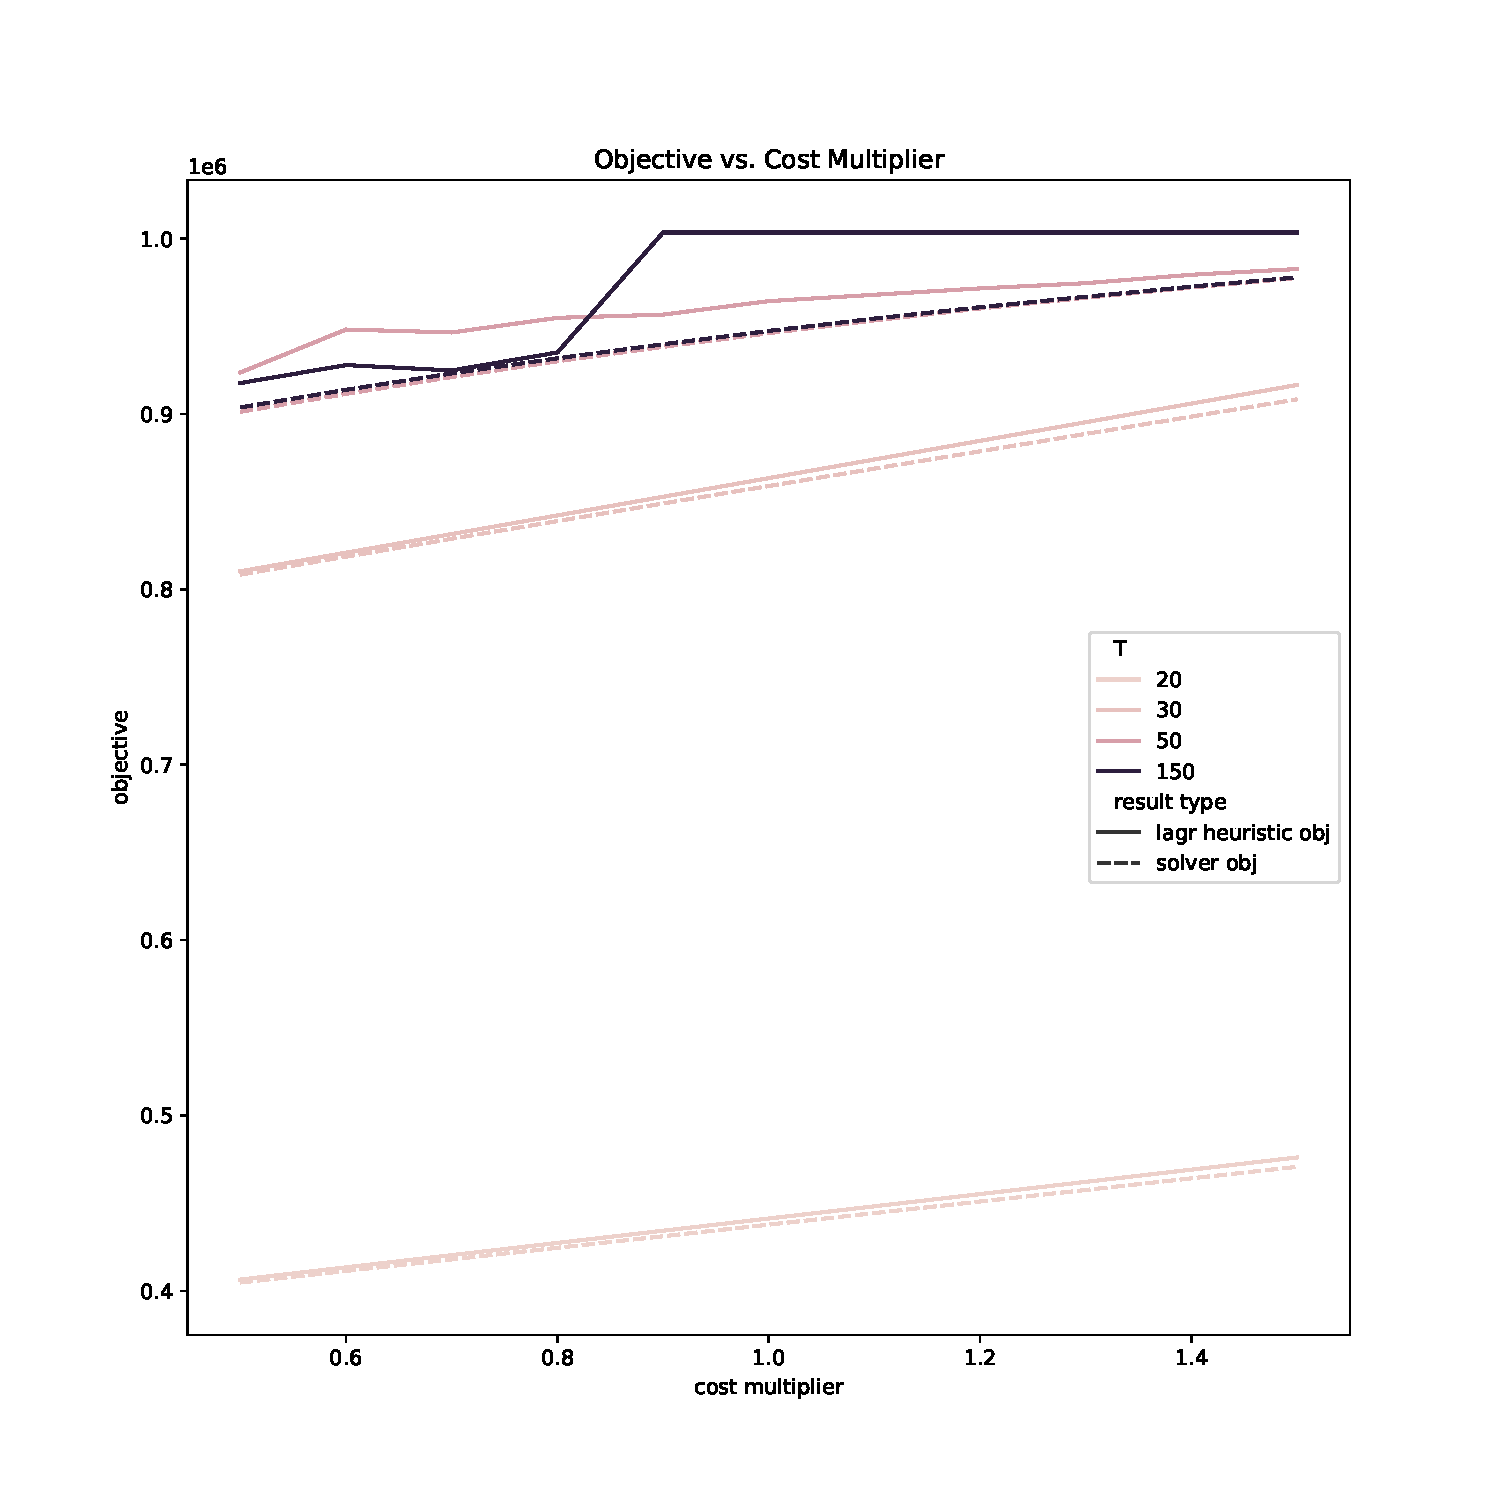
\includegraphics[width=0.45\linewidth]{figures/objective_vs_cost_multiplier.pdf}
    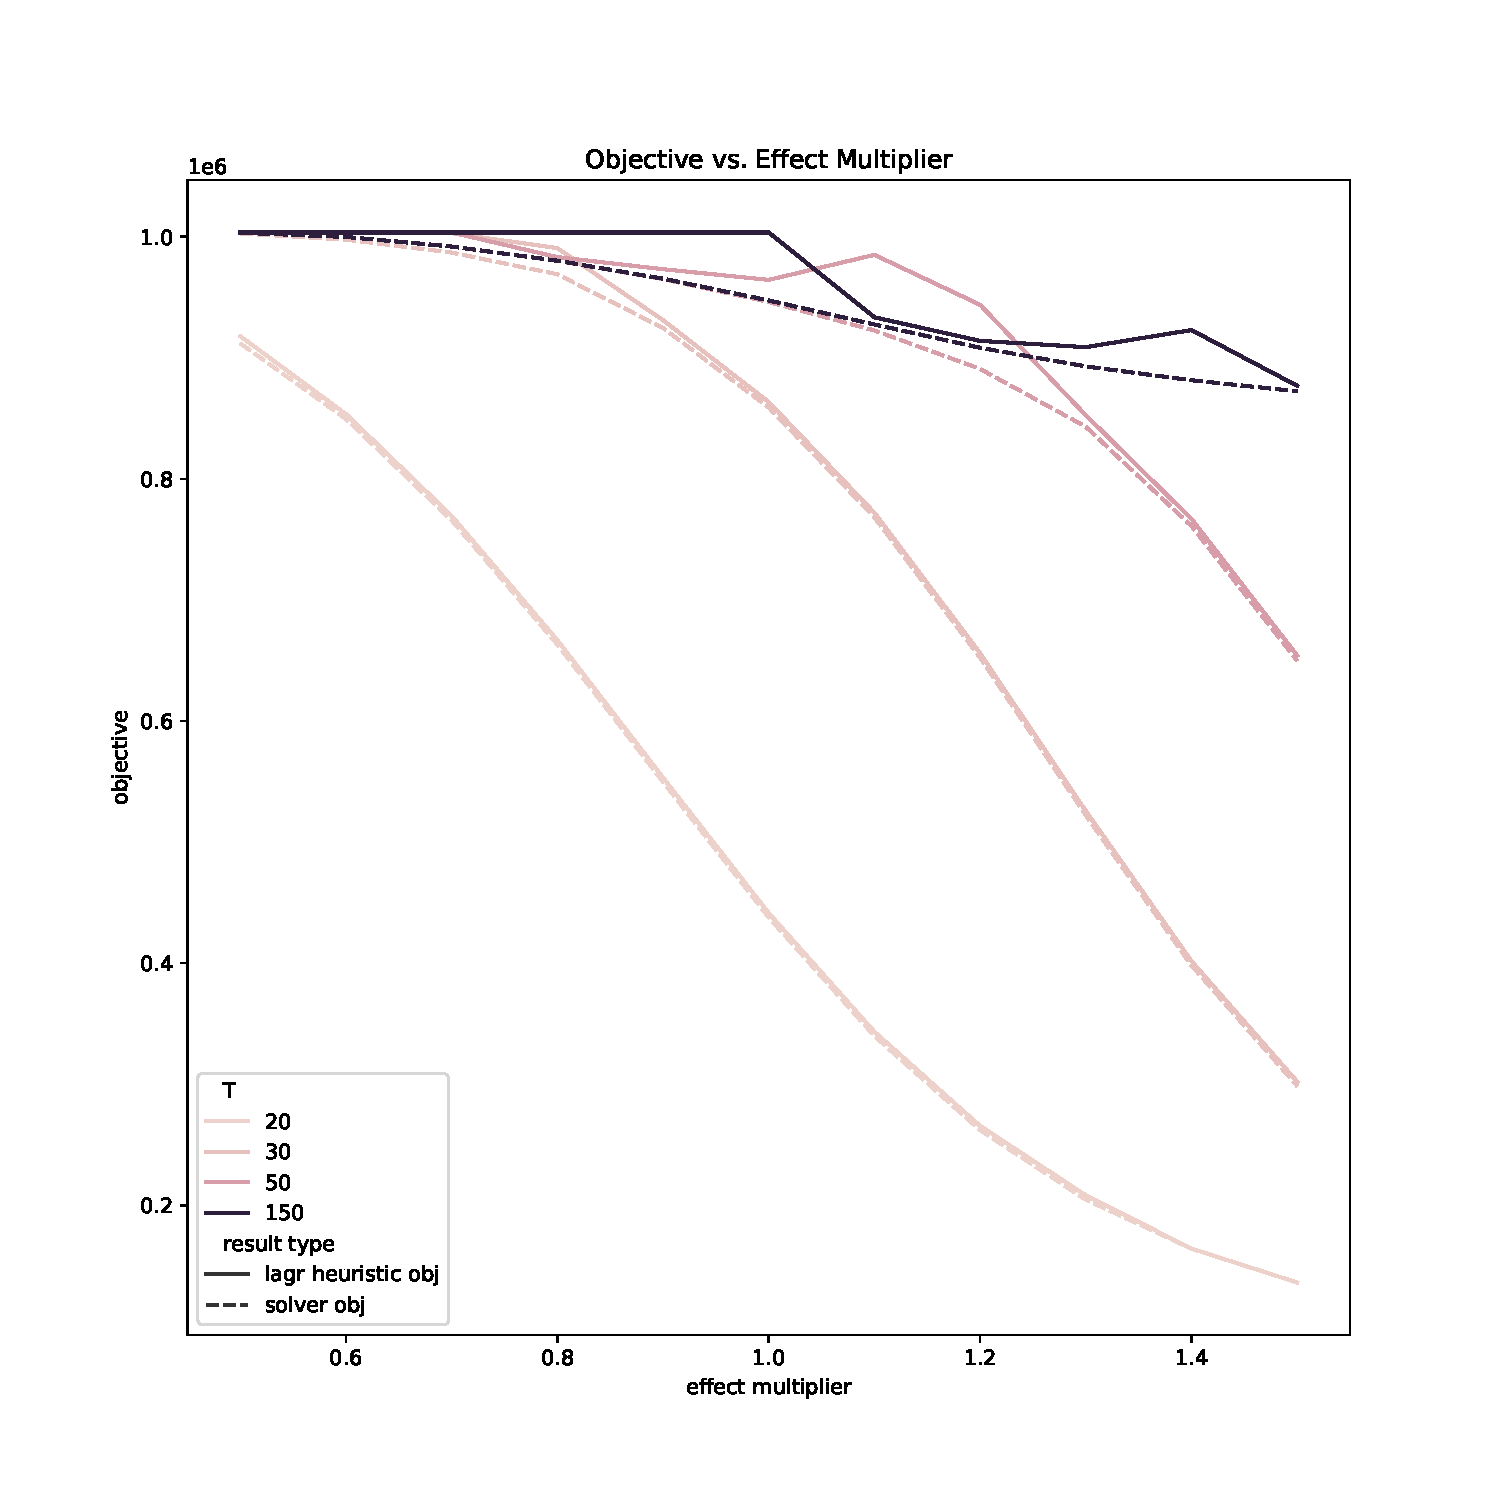
\includegraphics[width=0.45\linewidth]{figures/objective_vs_effect_multiplier.pdf}
    \caption{Objective value vs. factor by which policy costs are all changed; objective vs. factor by which policy effectivenesses are all changed.}
\end{figure}



\subsection{Lagrangian Subproblem Quasiconvexity}

The subproblem $L2(\lambda)$ defined in Section \ref{sec:lagrangian} has no integer constraints, but it still takes considerable time to solve with the BARON numerical solver. If the problem has suitable structure, such as quasiconvexity, a basic gradient descent algorithm might suffice for part of its solution. In particular, we examined whether $L2(\lambda)$ is quasiconvex in $P_t,t=1,\ldots,T$.

A function $f(\bm{x})$ is quasiconvex if and only if for any two values $\bm{x}_1$, and $\bm{x}_2$ in its domain, the function of one variable $V(\theta) = f((1-\theta)\bm{x}_1 + \theta\bm{x}_2)$ is quasiconvex for values of $\theta\in[0,1]$.

To probe this necessary and sufficient condition for quasiconvexity in $P$, we define the function $V_{P^1,P^2}:[0,1]\rightarrow \R$ for any values $P^1, P^2$ where $P^1_t$ and $P^2_t$ are fixed for all $t=1,\ldots,T$. This function is such that $V_{P^1, P^2}(\theta)$ is the optimal value of $L2(\lambda)$ where $P_t = (1-\theta) P^1_t + \theta P^2_t$ for all $t=1,\ldots,T$.

The following plots illustrate the value of $V_{P^1,P^2}(\theta)$ for $\theta\in[0,1]$. If the curves appear quasiconvex, then a necessary condition is met for $L2(\lambda)$ being quasiconvex in $P$. In each trial, the values $P^1_t, P^2_t,t=1,\ldots,T$ were generated in the interval $[0,1]$ uniformly randomly\footnote{In fact, for this model $P_t$ cannot be equal to $0$, because of its definition in the full model as a product of ``intervention effectiveness'' factors. So, the lowest value it can possibly take on is the product of the effectiveness factors of \emph{all} possible interventions. Both in the full model and in this investigation of quasiconvexity, values of $P_t$ are constrained to be in the interval $[P_{lb},1]$, where $P_{lb}$ is this small value. Since the logarithm of $P_t$ is part of the model, the domain becomes effectively open (the objective is undefined at $0$), this adjustment improves performance of the solver by giving a closed domain without loss of generality of solutions. The restriction of the domain for this quasiconvexity test is also without loss of generality, because for the purposes of this model, only values of $P_t$ in the constrained interval are relevant.}.

\begin{figure}[H]
    \center
    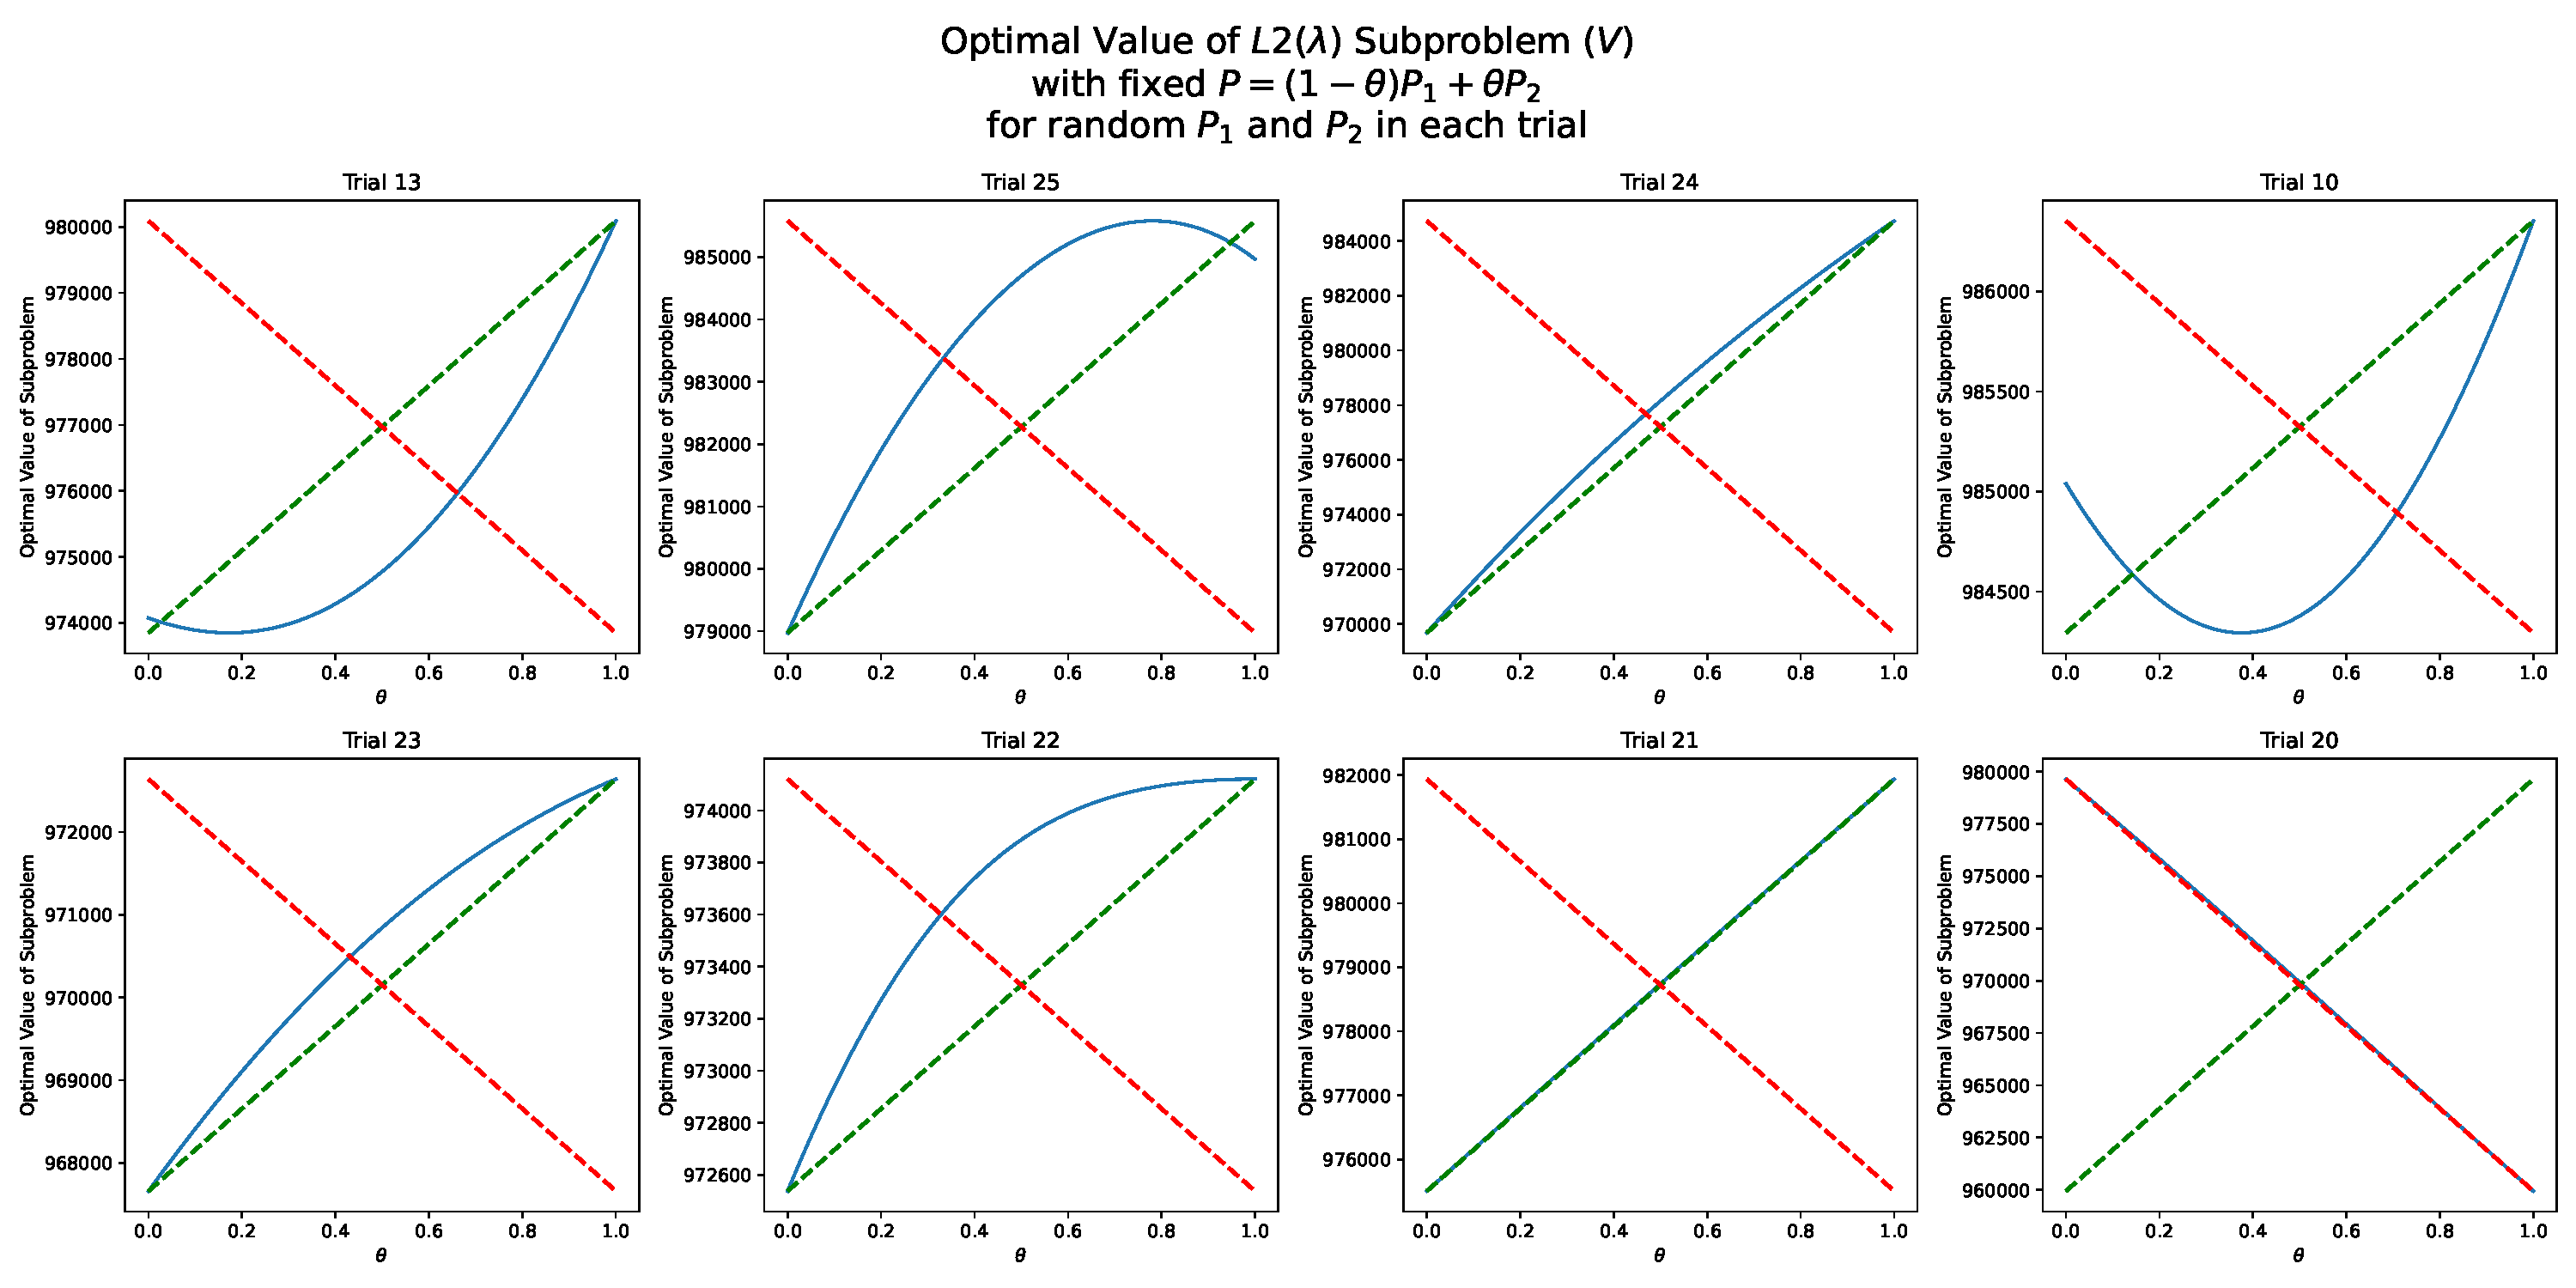
\includegraphics[width=\linewidth]{figures/L2_quasiconvexity_test.pdf}
    \caption{Optimal value of $L2(\lambda)$ with $P$ fixed to values that vary along a line; that is, $V_{P^1,P^2}(\theta)$ vs $\theta$ for several randomly-selected values of $P^1$ and $P^2$.}\label{fig:quasiconvexity_test}
\end{figure}

As can be seen in Figure \ref{fig:quasiconvexity_test}, the function $V$ appears to be neither quasiconvex nor quasiconcave.

To probe the possibility that the function $V$ is not jointly quasiconvex in the $P_t$ variables, but is componentwise quasiconvex in each $P_t,t=1,\ldots,P$, we can investigate whether the function $V_{P^1,P^2}(\theta)$ is quasiconvex for any $P^1,P^2$ such that the line segment connecting $P^1$ and $P^2$ is parallel to an axis $P_t$ (for some $t$), i.e. by repeating the same experiment but only varying one $P_t$ at a time.
\begin{figure}[H]
    \center
    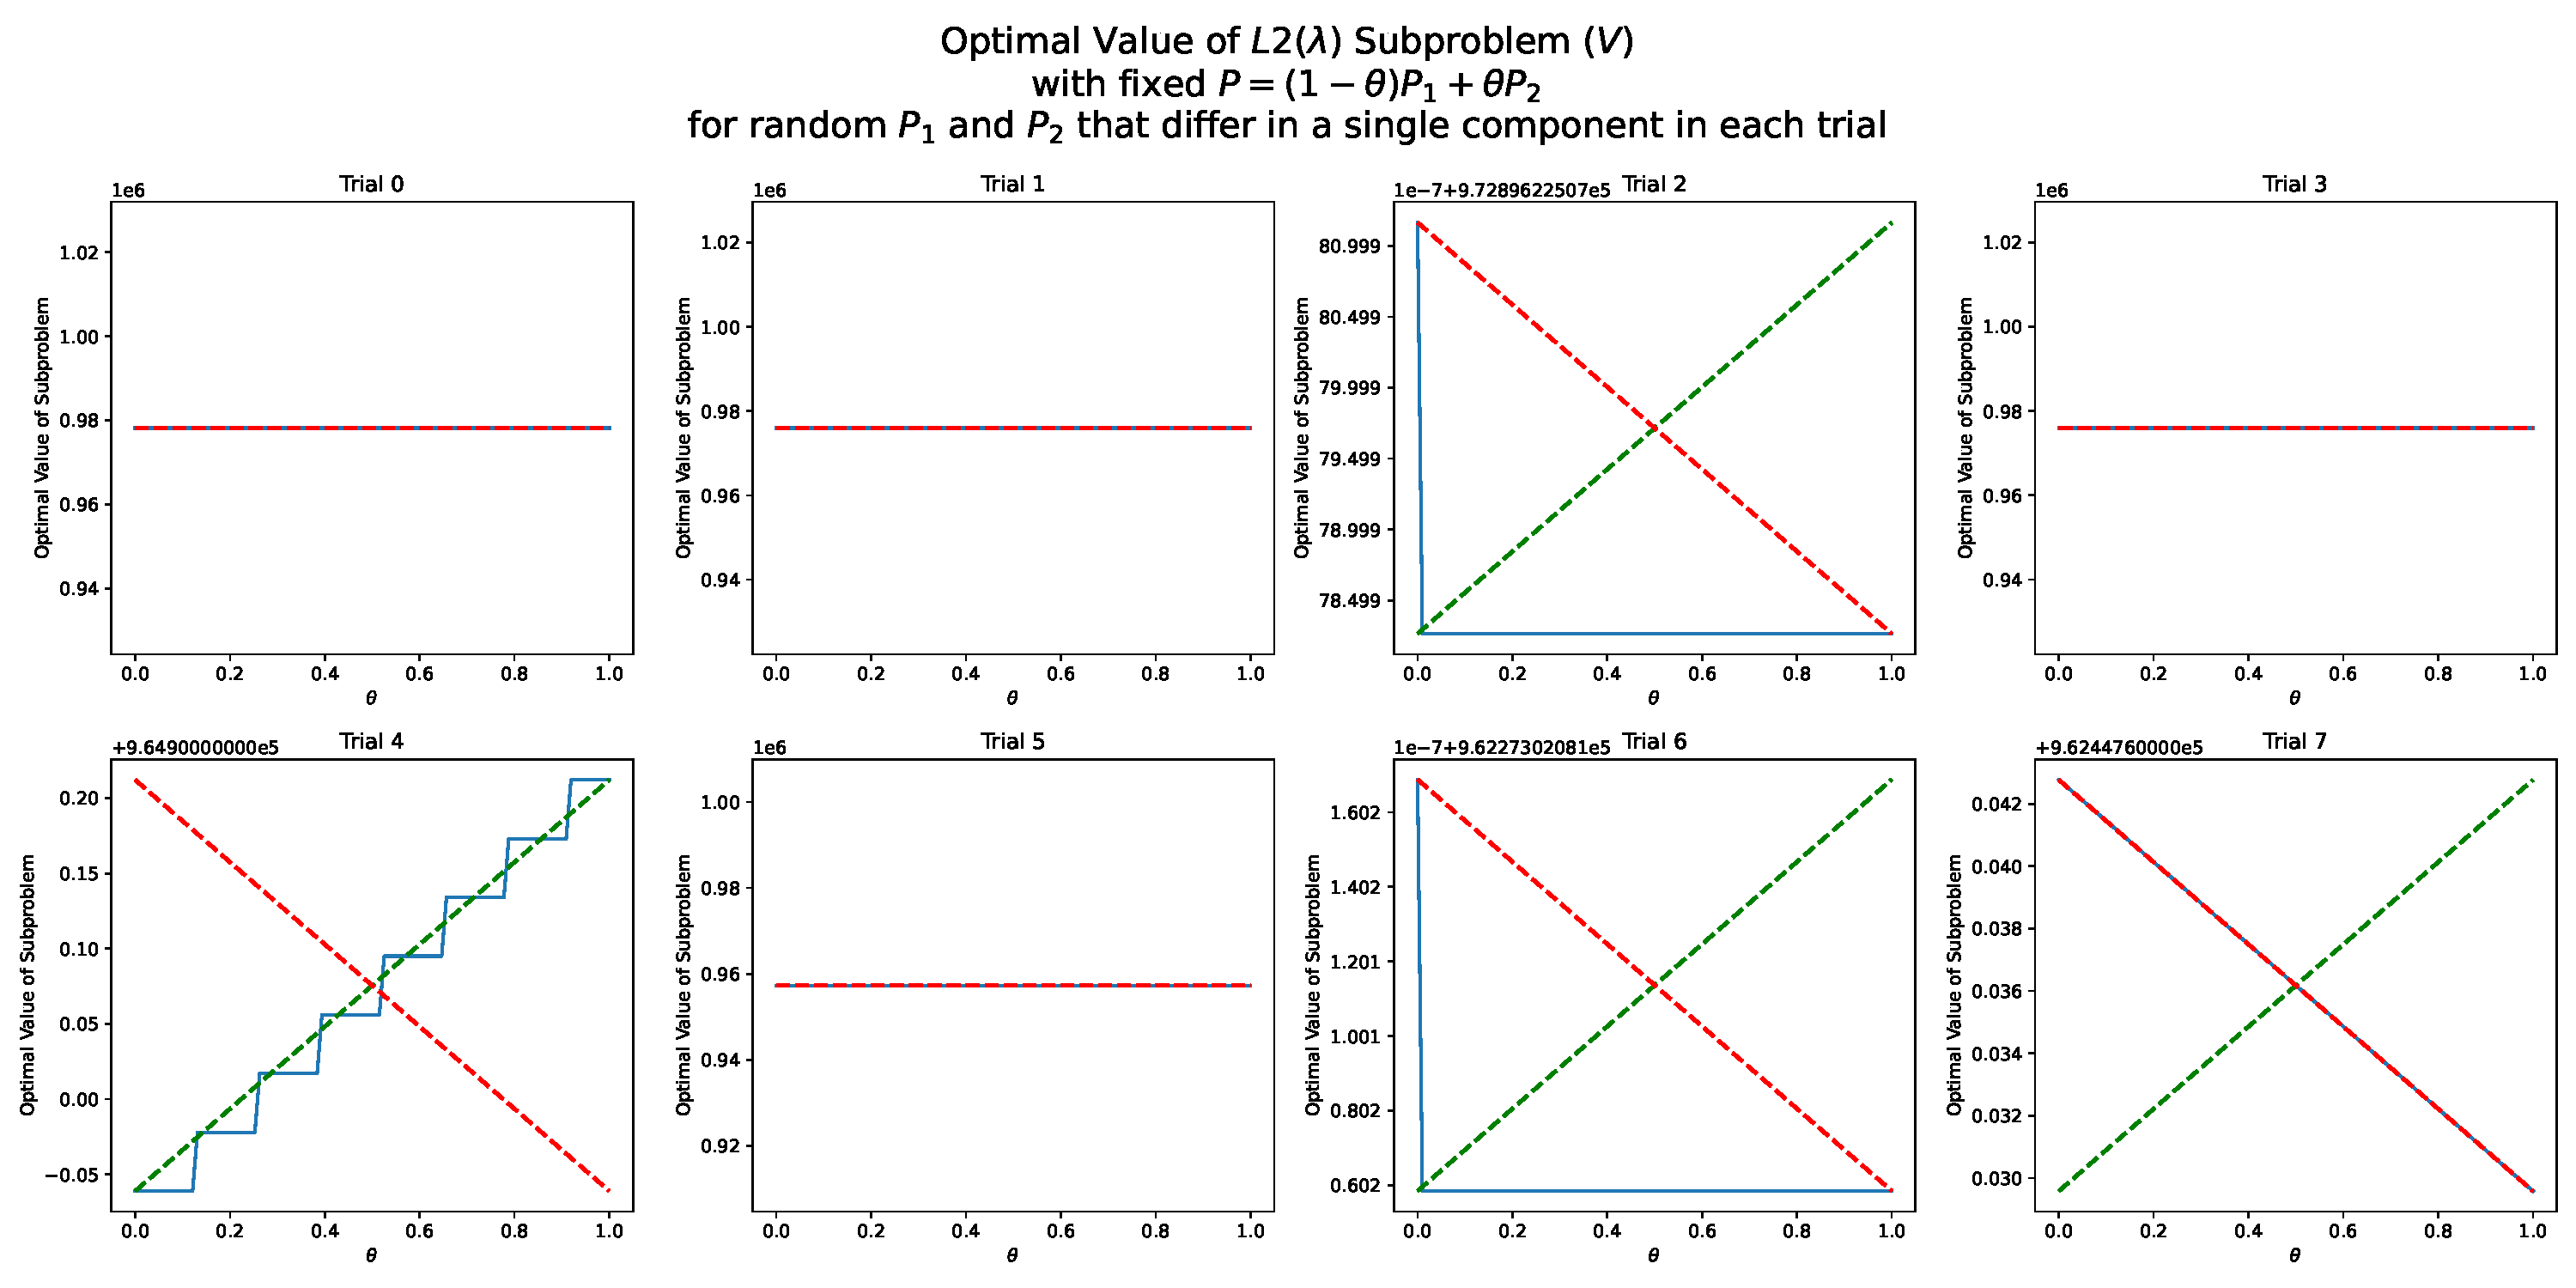
\includegraphics[width=\linewidth]{figures/L2_quasiconvexity_test_componentwise.pdf}
    \caption{The same experiment was repeated as is illustrated in Figure \ref{fig:quasiconvexity_test}, but by only varying a single $P_t$ component at a time.}\label{fig:quasiconvexity_test_componentwise}
\end{figure}

Based on the plots in Figure \ref{fig:quasiconvexity_test_componentwise}, it is inconclusive whether $V$ is componentwise quasiconcave or quasiconvex. The variation in the objective of the $L2(\lambda)$ subproblem may be small with respect to any one component $P_t$.



\section{Conclusion}



\newpage
\newpage
\bibliographystyle{plain}
\bibliography{bibliography.bib}
\nocite{*}
\end{document}




